\documentclass[
	article,
	11pt,
	oneside,
	a4paper,
	english,
	brazil,
	sumario=tradicional
]{abntex2}

\usepackage{lmodern}
\usepackage[T1]{fontenc}
\usepackage[utf8]{inputenc}
\usepackage{indentfirst}
\usepackage{nomencl}
\usepackage{color}
\usepackage{graphicx}
\usepackage{microtype}
\usepackage{lipsum}
\usepackage{dirtytalk}
\usepackage[brazilian,hyperpageref]{backref}
\usepackage[alf]{abntex2cite}

\titulo{Teste de usabilidade do primeiro protótipo da interface de usuário do \textit{Mercado Eletrônico para Transporte de Artefatos}}
\autor{Gabriel Pereira de Barros}
\local{Brasil}
\data{2017}

\definecolor{blue}{RGB}{41,5,195}
\makeatletter
\hypersetup{
	pdftitle={\@title},
	pdfauthor={\@author},
	pdfsubject={Teste de usabilidade do primeiro protótipo da interface de usuário do \textit{Mercado Eletrônico para Transporte de Artefatos}},
	pdfcreator={Criado com LaTeX e abnTeX2},
	pdfkeywords={teste de usabilidade}{interface de usuário}{mercado eletrônico}{logística de transportes},
	colorlinks=true,
	linkcolor=blue,
	citecolor=blue,
	filecolor=magenta,
	urlcolor=blue,
	bookmarksdepth=4
}
\makeatother
\makeindex

\setlrmarginsandblock{3cm}{3cm}{*}
\setulmarginsandblock{3cm}{3cm}{*}
\checkandfixthelayout
\setlength{\parindent}{1.3cm}
\setlength{\parskip}{0.2cm}
\SingleSpacing

\begin{document}
\selectlanguage{brazil}
\frenchspacing
\maketitle

\begin{resumoumacoluna}

	Este artigo pretende demonstrar o planejamento, o desenvolvimento e os resultados obtidos com a realização do primeiro teste de usabilidade da interface de usuário do sistema de informação, atualmente em desenvolvimento, denominado \textit{Mercado Eletrônico para Transporte de Artefatos}, realizado na disciplina de Interação Humano-Computador, ministrada pelo professor doutor Thiago Schumacher Barcelos, compondo assim o conjunto de artefatos, que em sua totalidade, representam o trabalho de conclusão de curso, necessário para a obtenção do grau de Tecnólogo em Análise e Desenvolvimento de Sistemas, pelo Instituto Federal de Ciência e Tecnologia de São Paulo, Campus Guarulhos. 
	
	\vspace{\onelineskip}
	\noindent

	\textbf{Palavras-chave}: teste de usabilidade, interface de usuário, mercado eletrônico, logística de transportes.
\end{resumoumacoluna}

\textual
\pagebreak

\renewcommand{\contentsname}{SUMÁRIO}

\pdfbookmark[0]{\contentsname}{toc}
\tableofcontents*
\cleardoublepage

\section*{Definição de teste de usabilidade}
	\addcontentsline{toc}{section}{Definição de teste de usabilidade}
	
	O teste de usabilidade é uma técnica utilizada no desenvolvimento de interfaces de sistemas de informação, cujo o objetivo é observar os potenciais usuários do sistema utilizando o produto para descobrir erros e pontos a serem melhorados. O produto pode ser um site, um sistema de informação ou, até mesmo, um produto físico, já que esta técnica pode ser aplicada em diferentes áreas. Protótipos são comumente utilizados para a realização desses testes \cite{usabilidade-na-web}.
	
	Os integrantes do teste de usabilidade são; o participante e o moderador. O participante tenta realizar as tarefas propostas pelo moderador, e enquanto o participante realiza a tentativa, o moderador registra os passos percorridos e as dificuldades enfrentadas pelo participante. No início de cada teste, o moderador deve descrever detalhadamente ao participante os objetivos a serem atingidos \cite{usabilidade-na-web}.
	
	O ambiente no qual se realiza o teste pode variar \cite{usabilidade-na-web}, mas o ideal é que ele seja feito no ambiente em que o sistema de informação será utilizado no dia a dia, para melhor ambientação do moderador e para aumentar a sua sensibilidade a questões relevantes ao projeto da interface de usuário. Podem haver problemas ao optar por realizar o teste do sistema de informação no ambiente no qual ele será utilizado, mas o objetivo é justamente este, identificar pontos de melhoria e pontos a serem corrigidos.
	
\vspace*{\fill}
\pagebreak

\section*{Identificação do sistema de informação a ser avaliado}
	\addcontentsline{toc}{section}{Identificação do sistema de informação a ser avaliado}
	
	A intensidade e a amplitude da utilização de aplicativos de entregas modificaram a forma como clientes de lojas virtuais e restaurantes realizam seus pedidos, bem como a relação trabalhista entre entregadores de objetos e o número de clientes captados por empresas de transporte.

	Esse processo prega, de forma indireta e implícita, a substituição e a obsolescência de postos de trabalho, e quem não se adapta a esta nova realidade sofre com prejuízos financeiros ou padece no desemprego, sem alcançar perspectivas melhores de vida. Além disso, a ideia da modalidade de trabalho pregada por esses aplicativos muitas vezes não convergem com o entendimento sobre vínculo empregatício dos trabalhadores brasileiros, altamente fundamentado na Consolidação das Leis do Trabalho (CLT).

	O \textit{Mercado Eletrônico para Transporte de Artefatos}, citado neste trabalho acadêmico, tem o objetivo de fazer a comunicação entre clientes, empresas de transporte e entregadores, sem promover uma modificação drástica na relação empregatícia estabelecida por esses dois últimos atores, mas apenas fortalecendo sua relação e aumentando os ganhos financeiros de todas as partes envolvidas e dando mais opções para os que necessitam transportar objetos. Este mercado eletrônico irá permitir o cadastro de clientes que necessitam realizar entregas e de prestadores desse serviço, como empresas de entregas e entregadores autônomos.

	No mundo real, o transporte de objetos pode envolver um ou mais pontos, sendo que nesses pontos objetos serão retirados ou entregues. O mercado eletrônico, ao final de seu desenvolvimento, irá contar com essa funcionalidade, permitindo que o cliente também informe as dimensões dos objetos e seus respectivos pesos, selecionando o entregador mais próximo do primeiro ponto que possua um veículo apto a transportar esses objetos. Não haverá limites para o cadastro de pontos e objetos, desde que sejam encontrados entregadores aptos a realizar o transporte.

	A plataforma irá contar com sistema de saldo virtual, sendo esse alimentado por meio de depósitos com boletos bancários. O pagamento dos pedidos será realizado através de débito em saldo ou em dinheiro, de forma presencial. Somente os entregadores que contam com saldo em conta poderão aceitar pedidos em que o pagamento será realizado em dinheiro. Uma pequena parte do valor do pedido será utilizado para realizar manutenção na plataforma e o restante será repassado para os prestadores, que poderão realizar o saque do lucro obtido através de moedas virtuais ou utilizar esse valor para promover seus serviços através de priorização na busca de prestadores.
	
\vspace*{\fill}
\pagebreak

\section*{Identificação do experimento}
	\addcontentsline{toc}{section}{Identificação do experimento}
	
	Para a realização do teste de usabilidade, foram definidas três atividades sequenciais, que são triviais para a realização do propósito geral do sistema de informação; a definição de um ponto de retirada de um objeto, a definição de um ponto de entrega de um objeto e a alteração dos dados de um ponto de retirada, respectivamente.
	
	O moderador deve preparar o ambiente de testes, incluindo o acesso ao sítio eletrônico e a realização da autenticação na plataforma, relatar ao participante os objetivos a serem atingidos e registrar as atitudes tomadas, as dificuldades enfrentadas e as sugestões indicadas pelo mesmo.
	
	A seguir, as características de cada uma das tarefas serão descritas detalhadamente, com a inclusão de capturas de tela do estado da interface de usuário esperadas, antes, durante e depois da interação de um potencial usuário:
	
	\begin{enumerate}
		\item Definição de um ponto de retirada de um objeto.
		
		Nesta atividade, o usuário deve definir um ponto de retirada de um objeto, com o endereço na \say{\textit{Rua da Creche, 206 - Jardim Guaracy, Guarulhos - SP, Brasil}}, sem complemento, o mensageiro deve \say{\textit{retirar uma caixa com livros}}, quando chegar neste local, e o e-mail a ser notificado quando isso acontecer é o \say{\textit{contato@pereirabarros.com}}.
		
		Os estados esperados para a interface de usuário, antes, durante e depois da interação, podem ser visualizados nas figuras \ref{fig:antes-retirada}, \ref{fig:durante-retirada} e \ref{fig:depois-retirada}, respectivamente.
		
		\item Definição de um ponto de entrega de um objeto.
		
		Nesta atividade, o usuário deve definir um ponto de entrega de um objeto, com o endereço na \say{\textit{Rua do Esporte, 210 - Jardim Guaracy, Guarulhos - SP, Brasil}}, sem complemento, o mensageiro deve \say{\textit{entregar uma caixa com livros}}, quando chegar neste local, e o e-mail a ser notificado quando isso acontecer é o \say{\textit{opereirabarros@outlook.com}}.
		
		Os estados esperados para a interface de usuário, antes, durante e depois da interação, podem ser visualizados nas figuras \ref{fig:antes-entrega}, \ref{fig:durante-entrega} e \ref{fig:depois-entrega}, respectivamente.
		
		\item Alteração dos dados de um ponto de retirada.
		
		Nesta atividade, o usuário deve alterar os dados de um ponto de retirada, com a especificação do endereço \say{\textit{Avenida Paulista, 1110 - Bela Vista, São Paulo - SP, Brasil}}, sem complemento, o mensageiro deve \say{\textit{retirar um conjunto de caixas que contém livros}}, quando chegar neste local, e o e-mail a ser notificado quando isso acontecer é o \say{\textit{pereira.barros.contato@gmail.com}}.
		
		Os estados esperados para a interface de usuário, antes, durante e depois da interação, podem ser visualizados nas figuras \ref{fig:antes-alterar}, \ref{fig:durante-alterar} e \ref{fig:depois-alterar}, respectivamente.
		
	\end{enumerate}
	
\vspace*{\fill}
\pagebreak
	
\section*{Realização do experimento}
	\addcontentsline{toc}{section}{Realização do experimento}
	
	O único participante do teste de usabilidade da interface de usuário do \textit{Mercado Eletrônico para Transporte de Artefatos} se chama Gabriel de Souza Martins e nunca teve contato em um momento anterior com uma plataforma de entrega de objetos, sendo este o seu primeiro contato com uma ferramenta dessa categoria.
	
	Na realização da primeira atividade, o usuário mostrou-se proativo ao realizar o preenchimento dos campos em pouco tempo, mas ele se esqueceu apenas de informar o número predial, que compõe o endereço de retirada, mas logo percebeu esse equívoco, por que o sistema emitiu uma mensagem informando essa situação, conforme pode ser visualizado na figura \ref{fig:falta-numero}, corrigiu o erro e avançou para a próxima tela, que define a conclusão da tarefa, representada na figura \ref{fig:depois-retirada}.
	
	Na segunda atividade, a tela representada na figura \ref{fig:depois-retirada} já estava apresentada, então o usuário não precisou realizar nenhum passo adicional para acessá-la. Por conta da similaridade com a tela anterior, o usuário a preencheu tão rápido quanto a citada, mas desta vez não cometeu erros.
	
	Na realização da terceira atividade, referente a alteração dos dados do ponto de retirada, o usuário ficou em dúvida sobre qual botão deveria ser pressionado para realizar a atividade, ficando cerca de dez segundos a procura do botão \textit{editar}. Assim que o encontrou, pode realizar a alteração tranquilamente, sem maiores problemas.
	
	O usuário informou que a interface da plataforma é intuitiva e que os erros cometidos por ele poderiam ter sido prevenidos com a presença de um assistente (comumente conhecido como \textit{wizard}). Ele demonstrou curiosidade quando as outras telas que compõem a interface de usuário, o moderador mostrou-as para ele e esse reconheceu a presença de padrões na construção da interface, e disse que isso facilita o reconhecimento de funções.
	
\vspace*{\fill}
\pagebreak
	
\section*{Conclusão}
	\addcontentsline{toc}{section}{Conclusão}
	
	A partir dos resultados obtidos, pode-se perceber que a presença de um assistente, que guie o usuário na realização de atividades, com balões informativos e outros elementos que facilitem o reconhecimento de elementos, iria facilitar ainda mais a realização das atividades triviais do sistema, como a descrição dos dados de pontos e a edição dos mesmos.
	
	Parte da interface de usuário não está completa; na próxima etapa de desenvolvimento do sistema de informação, a equipe irá construir os elementos que compõem a tela de definição e associação de objetos aos pontos, com a especificação de suas dimensões e peso. Dar-se-á preferência para os princípios já estabelecidos e reconhecidos pelo participante do teste de usabilidade, que é a adoção de padrões na construção de interfaces, que proporcionam fácil reconhecimento de funções e promovem o autoaprendizado por parte dos usuários.
	
	Este foi o primeiro teste de usabilidade realizado para averiguar se as decisões tomadas na construção da interface de usuário foram bem-sucedidas, e pelo que constatou-se, elas o foram, parcialmente, se não fosse os erros cometidos pelo participante (ocasionados pela falta de um \textit{wizard}, segundo o mesmo). Obviamente, o presente teste de usabilidade, assim como futuros, devem ser realizados com uma qualidade maior de participantes, para tornar os parâmetros utilizados na tomada de decisões mais fidedignos e confiáveis.

\vspace*{\fill}
\pagebreak

\begin{apendicesenv}
\partapendices

\chapter{Estados da interface de usuário}
\label{apend:estados-interface}

		\begin{figure}[!h]
			\centering
			\caption{Estado da interface de usuário esperada antes da definição do ponto de retirada}
			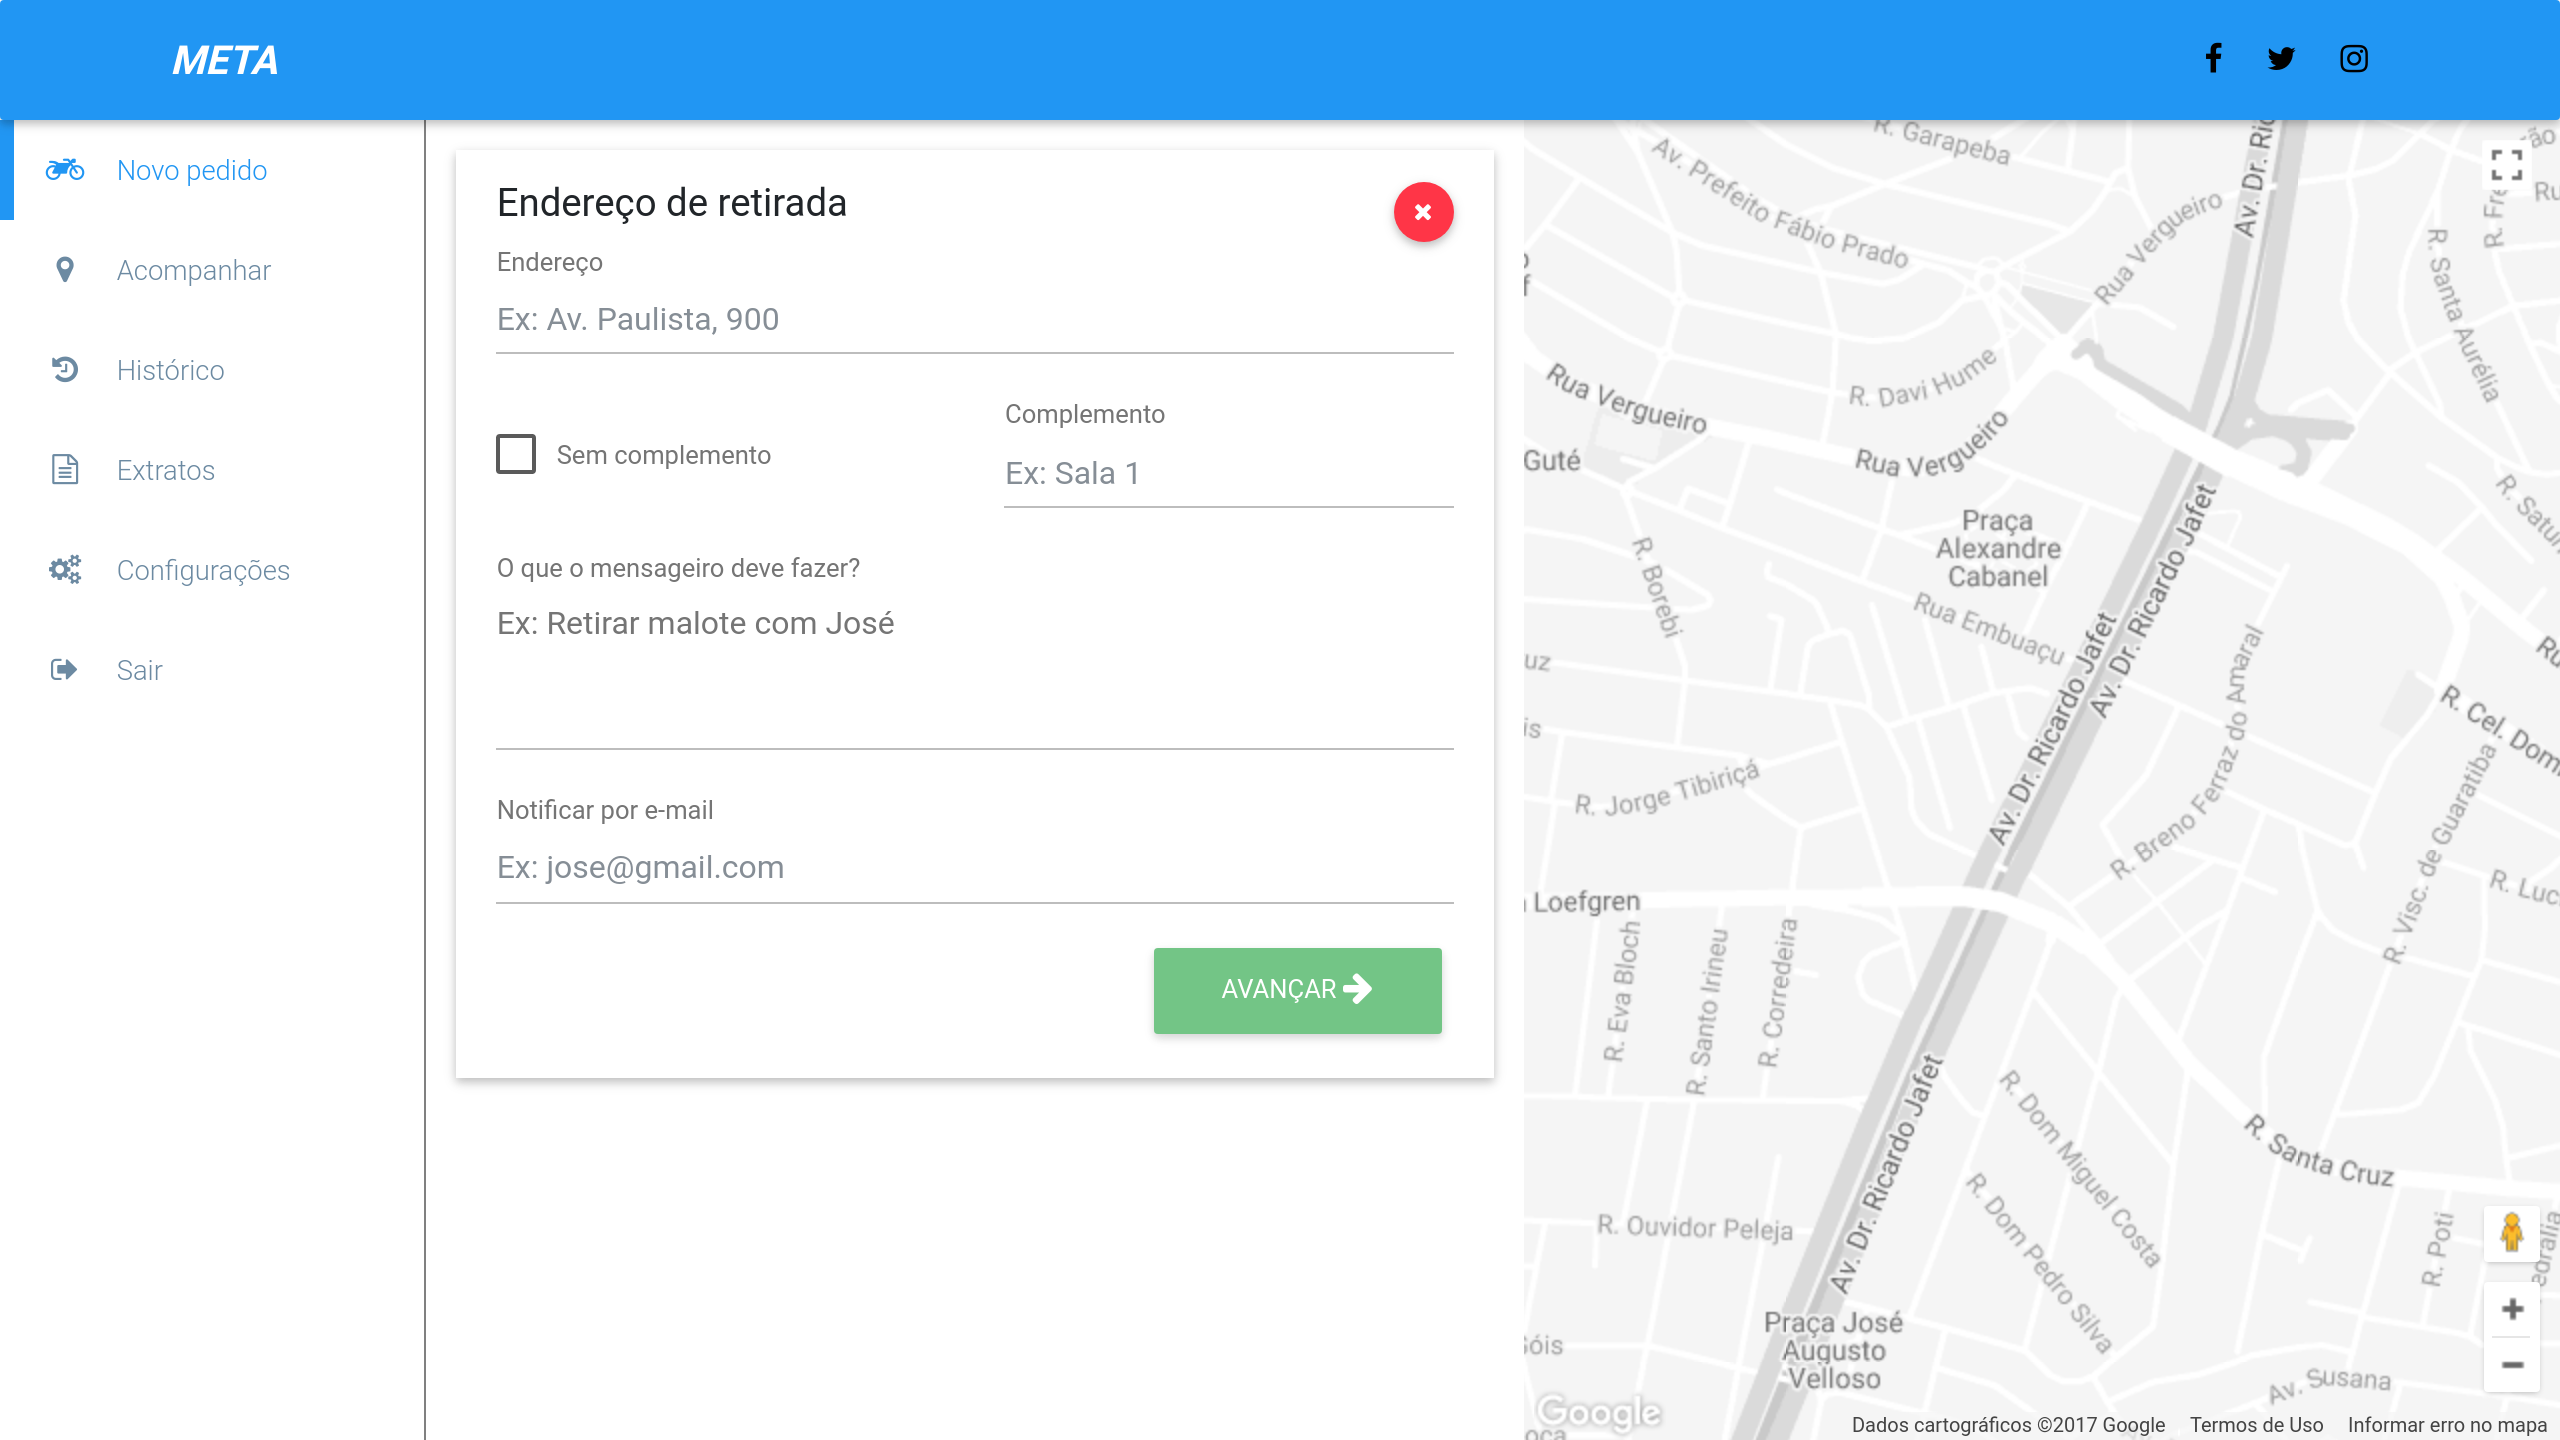
\includegraphics[width=1\textwidth]{./img/antes-retirada}
			\fonte{Captura de tela realizada pelo autor}
			\label{fig:antes-retirada}
		\end{figure}
		
		\begin{figure}[!h]
			\centering
			\caption{Estado da interface de usuário esperada durante da definição do ponto de retirada}
			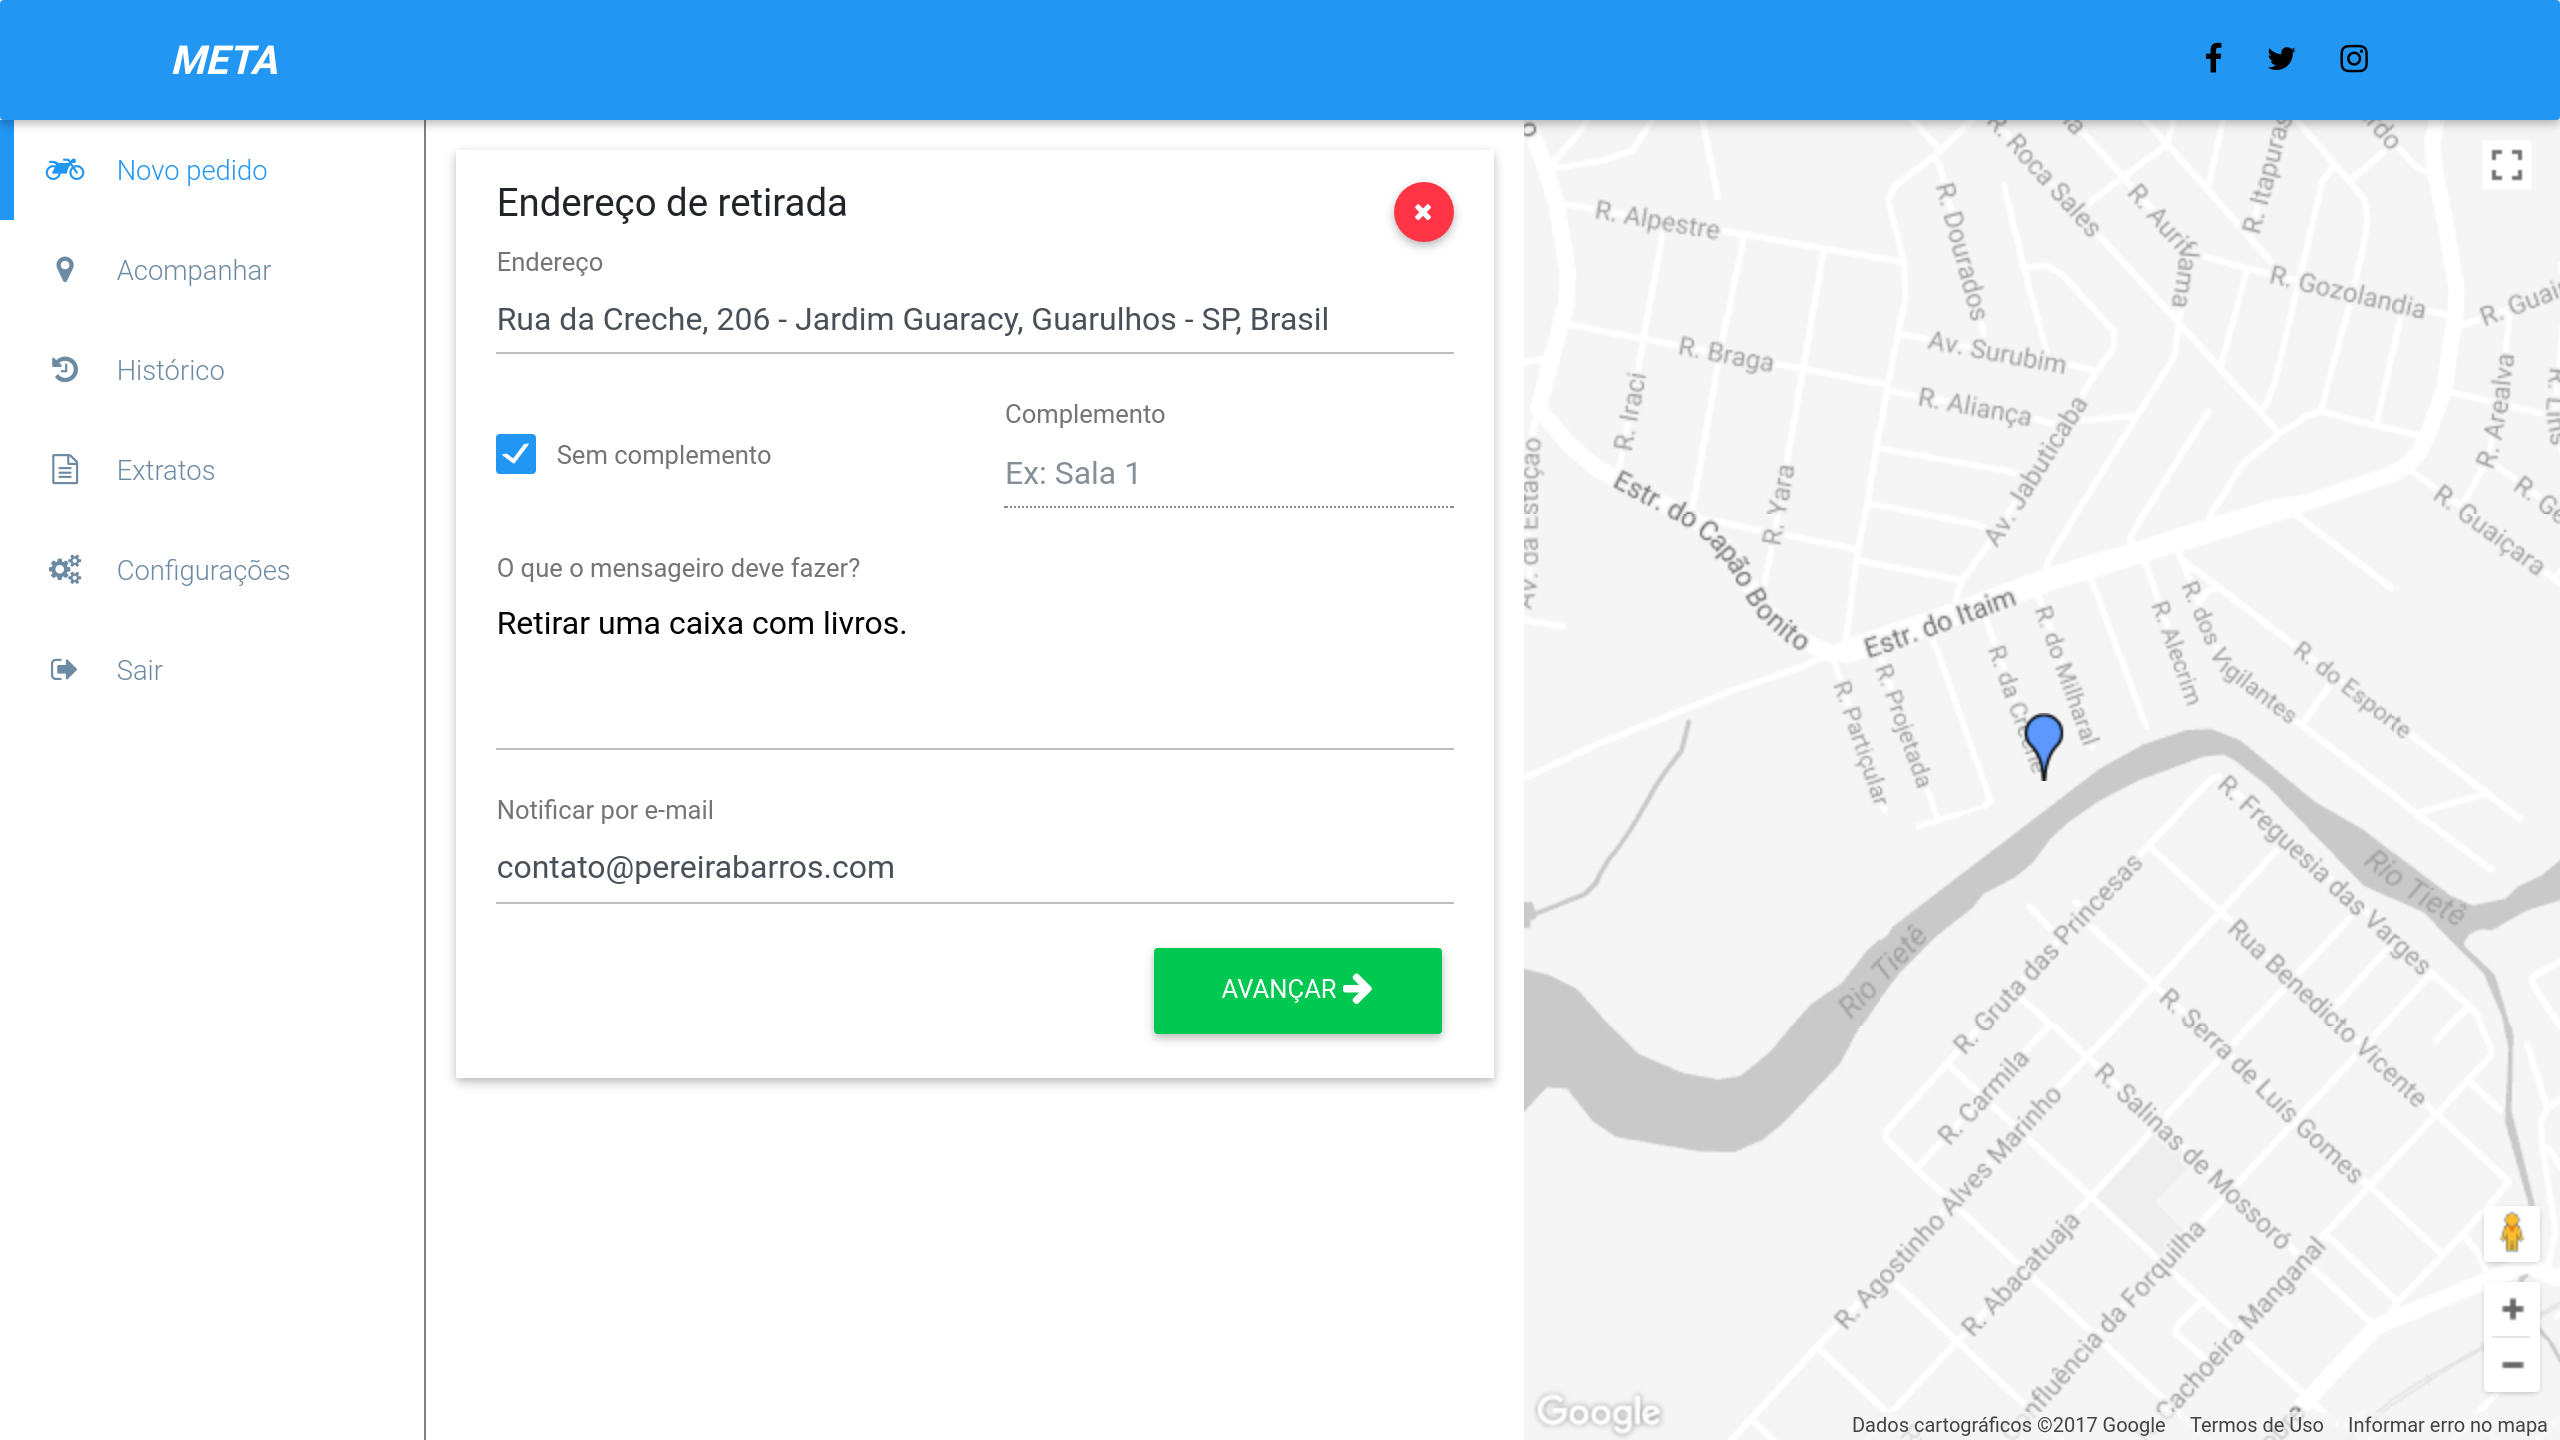
\includegraphics[width=1\textwidth]{./img/durante-retirada}
			\fonte{Captura de tela realizada pelo autor}
			\label{fig:durante-retirada}
		\end{figure}
		
		\begin{figure}[!h]
			\centering
			\caption{Estado da interface de usuário esperada depois da definição do ponto de retirada}
			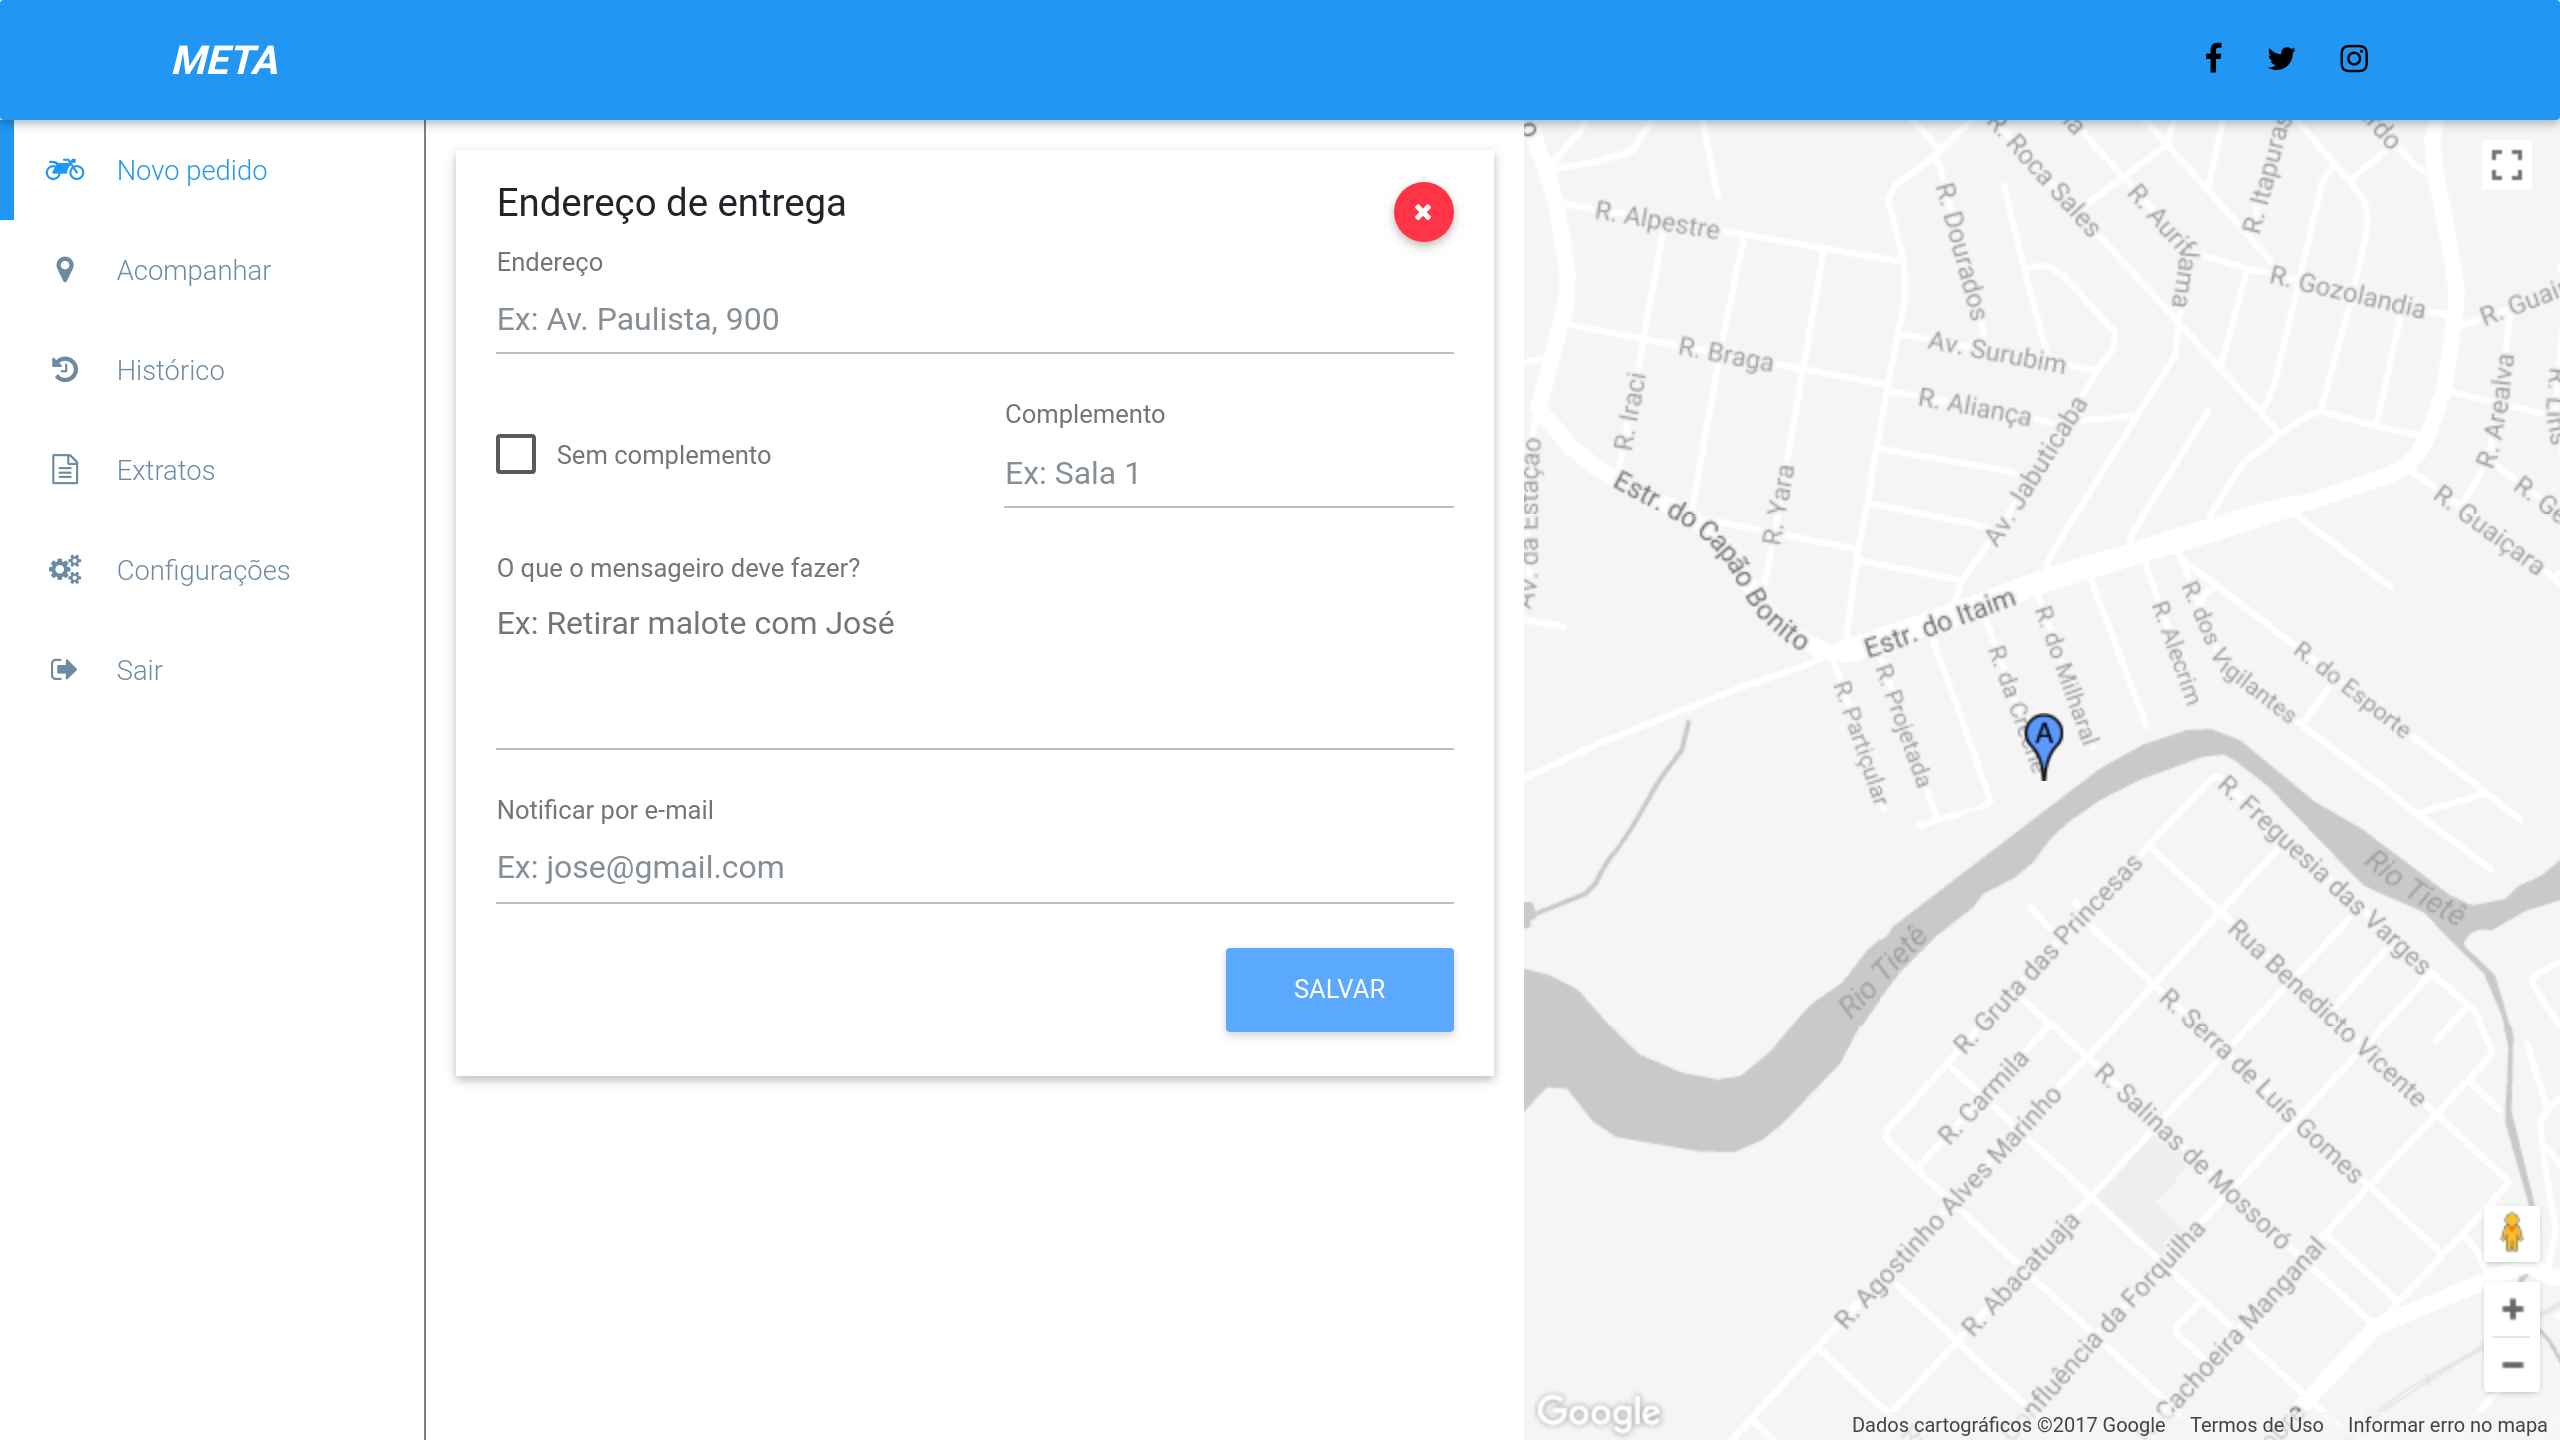
\includegraphics[width=1\textwidth]{./img/depois-retirada}
			\fonte{Captura de tela realizada pelo autor}
			\label{fig:depois-retirada}
		\end{figure}

		\begin{figure}[!h]
			\centering
			\caption{Estado da interface de usuário esperada antes da definição do ponto de entrega}
			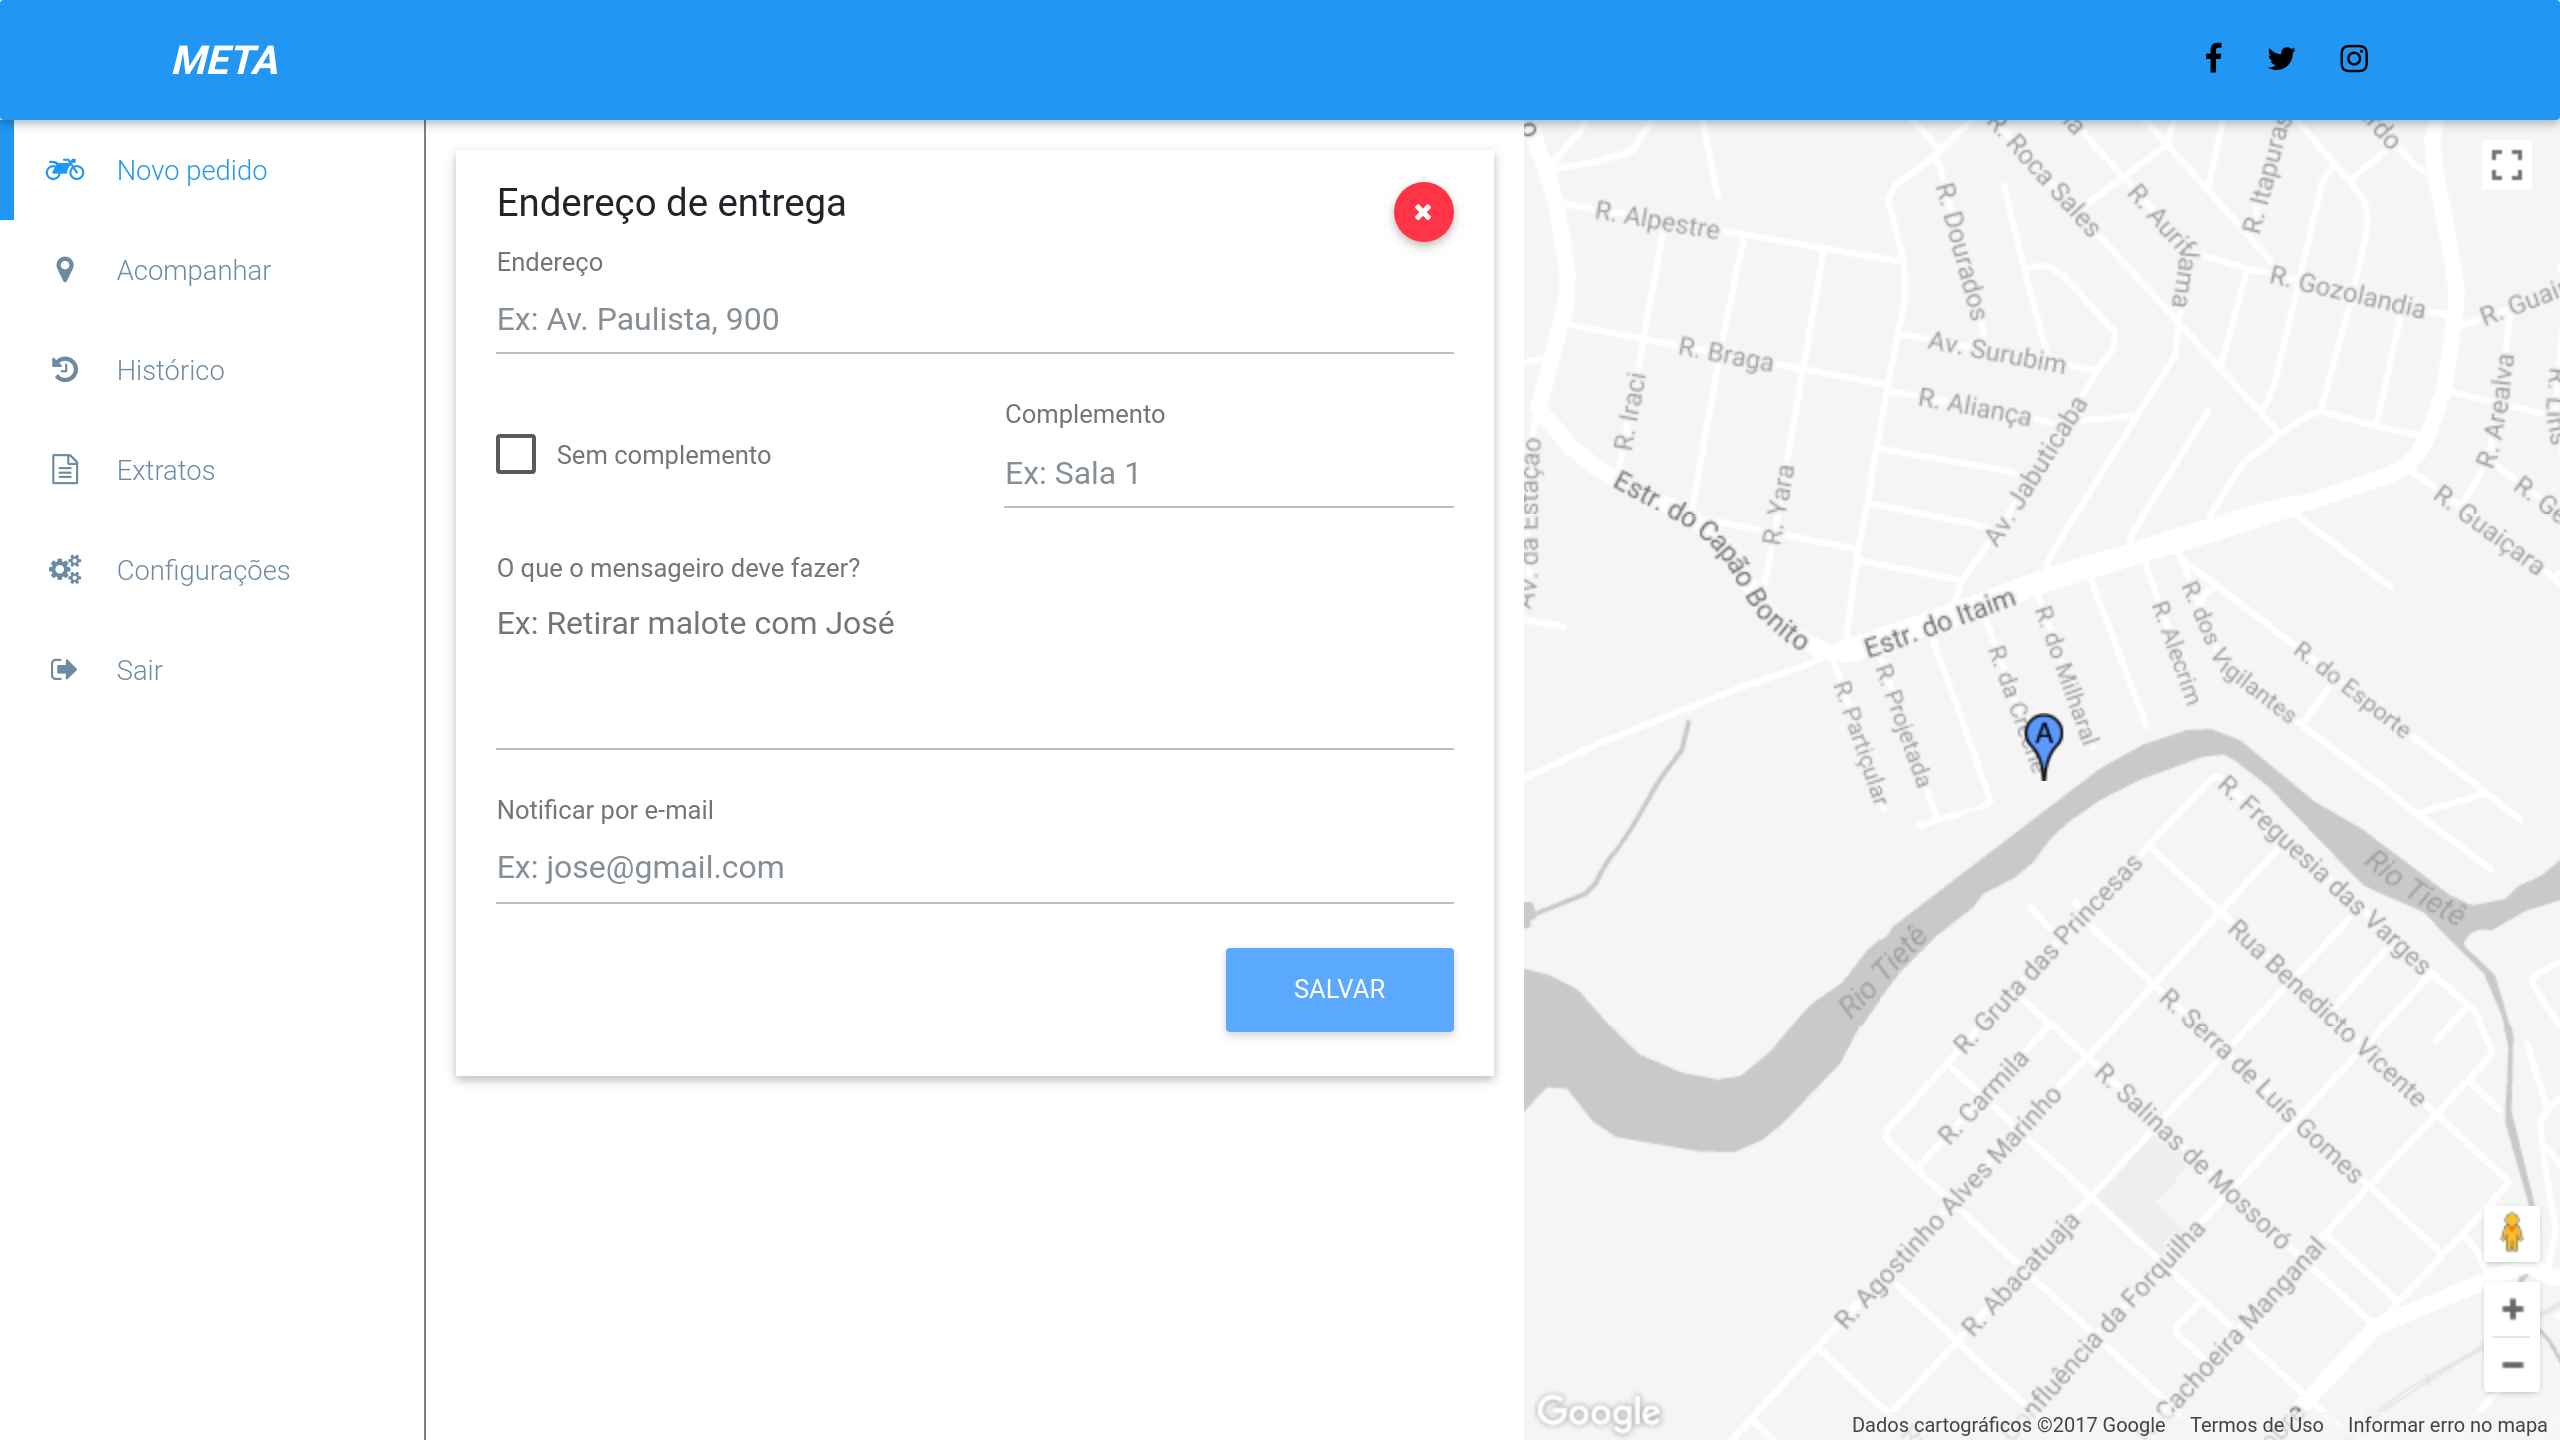
\includegraphics[width=1\textwidth]{./img/depois-retirada}
			\fonte{Captura de tela realizada pelo autor}
			\label{fig:antes-entrega}
		\end{figure}
		
		\begin{figure}[!h]
			\centering
			\caption{Estado da interface de usuário esperada durante da definição do ponto de entrega}
			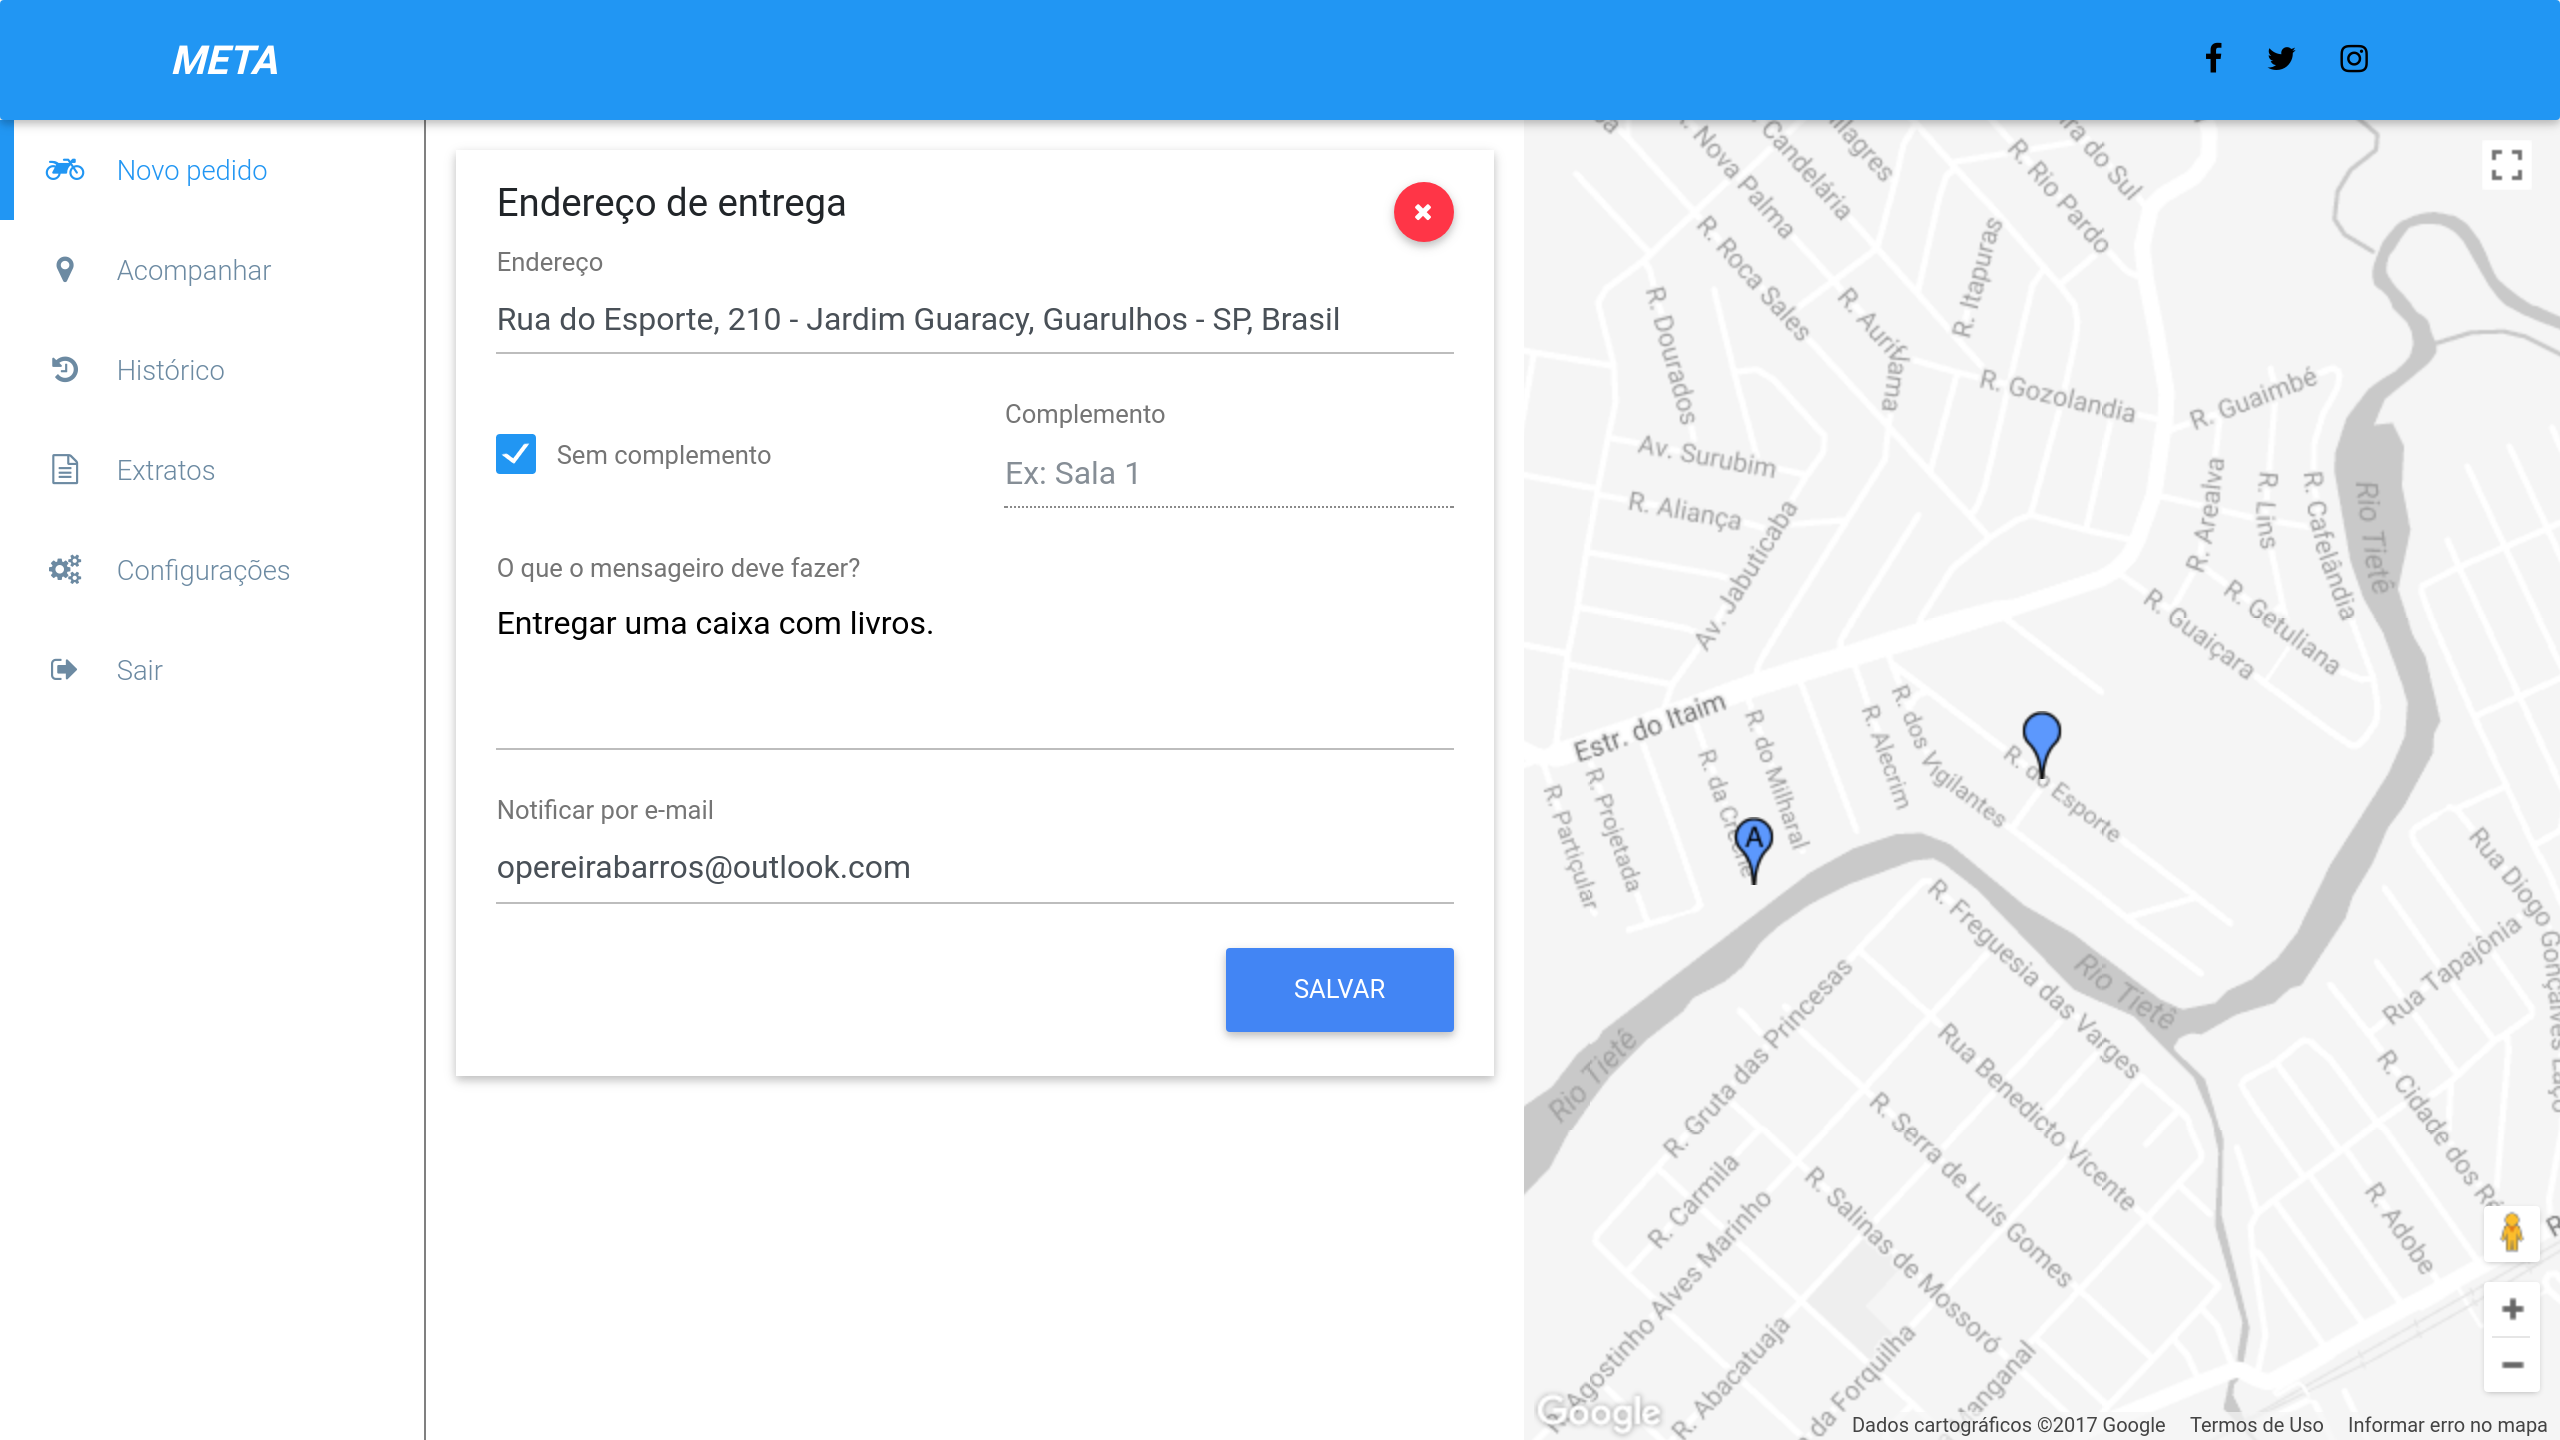
\includegraphics[width=1\textwidth]{./img/durante-entrega}
			\fonte{Captura de tela realizada pelo autor}
			\label{fig:durante-entrega}
		\end{figure}
		
		\begin{figure}[!h]
			\centering
			\caption{Estado da interface de usuário esperada depois da definição do ponto de entrega}
			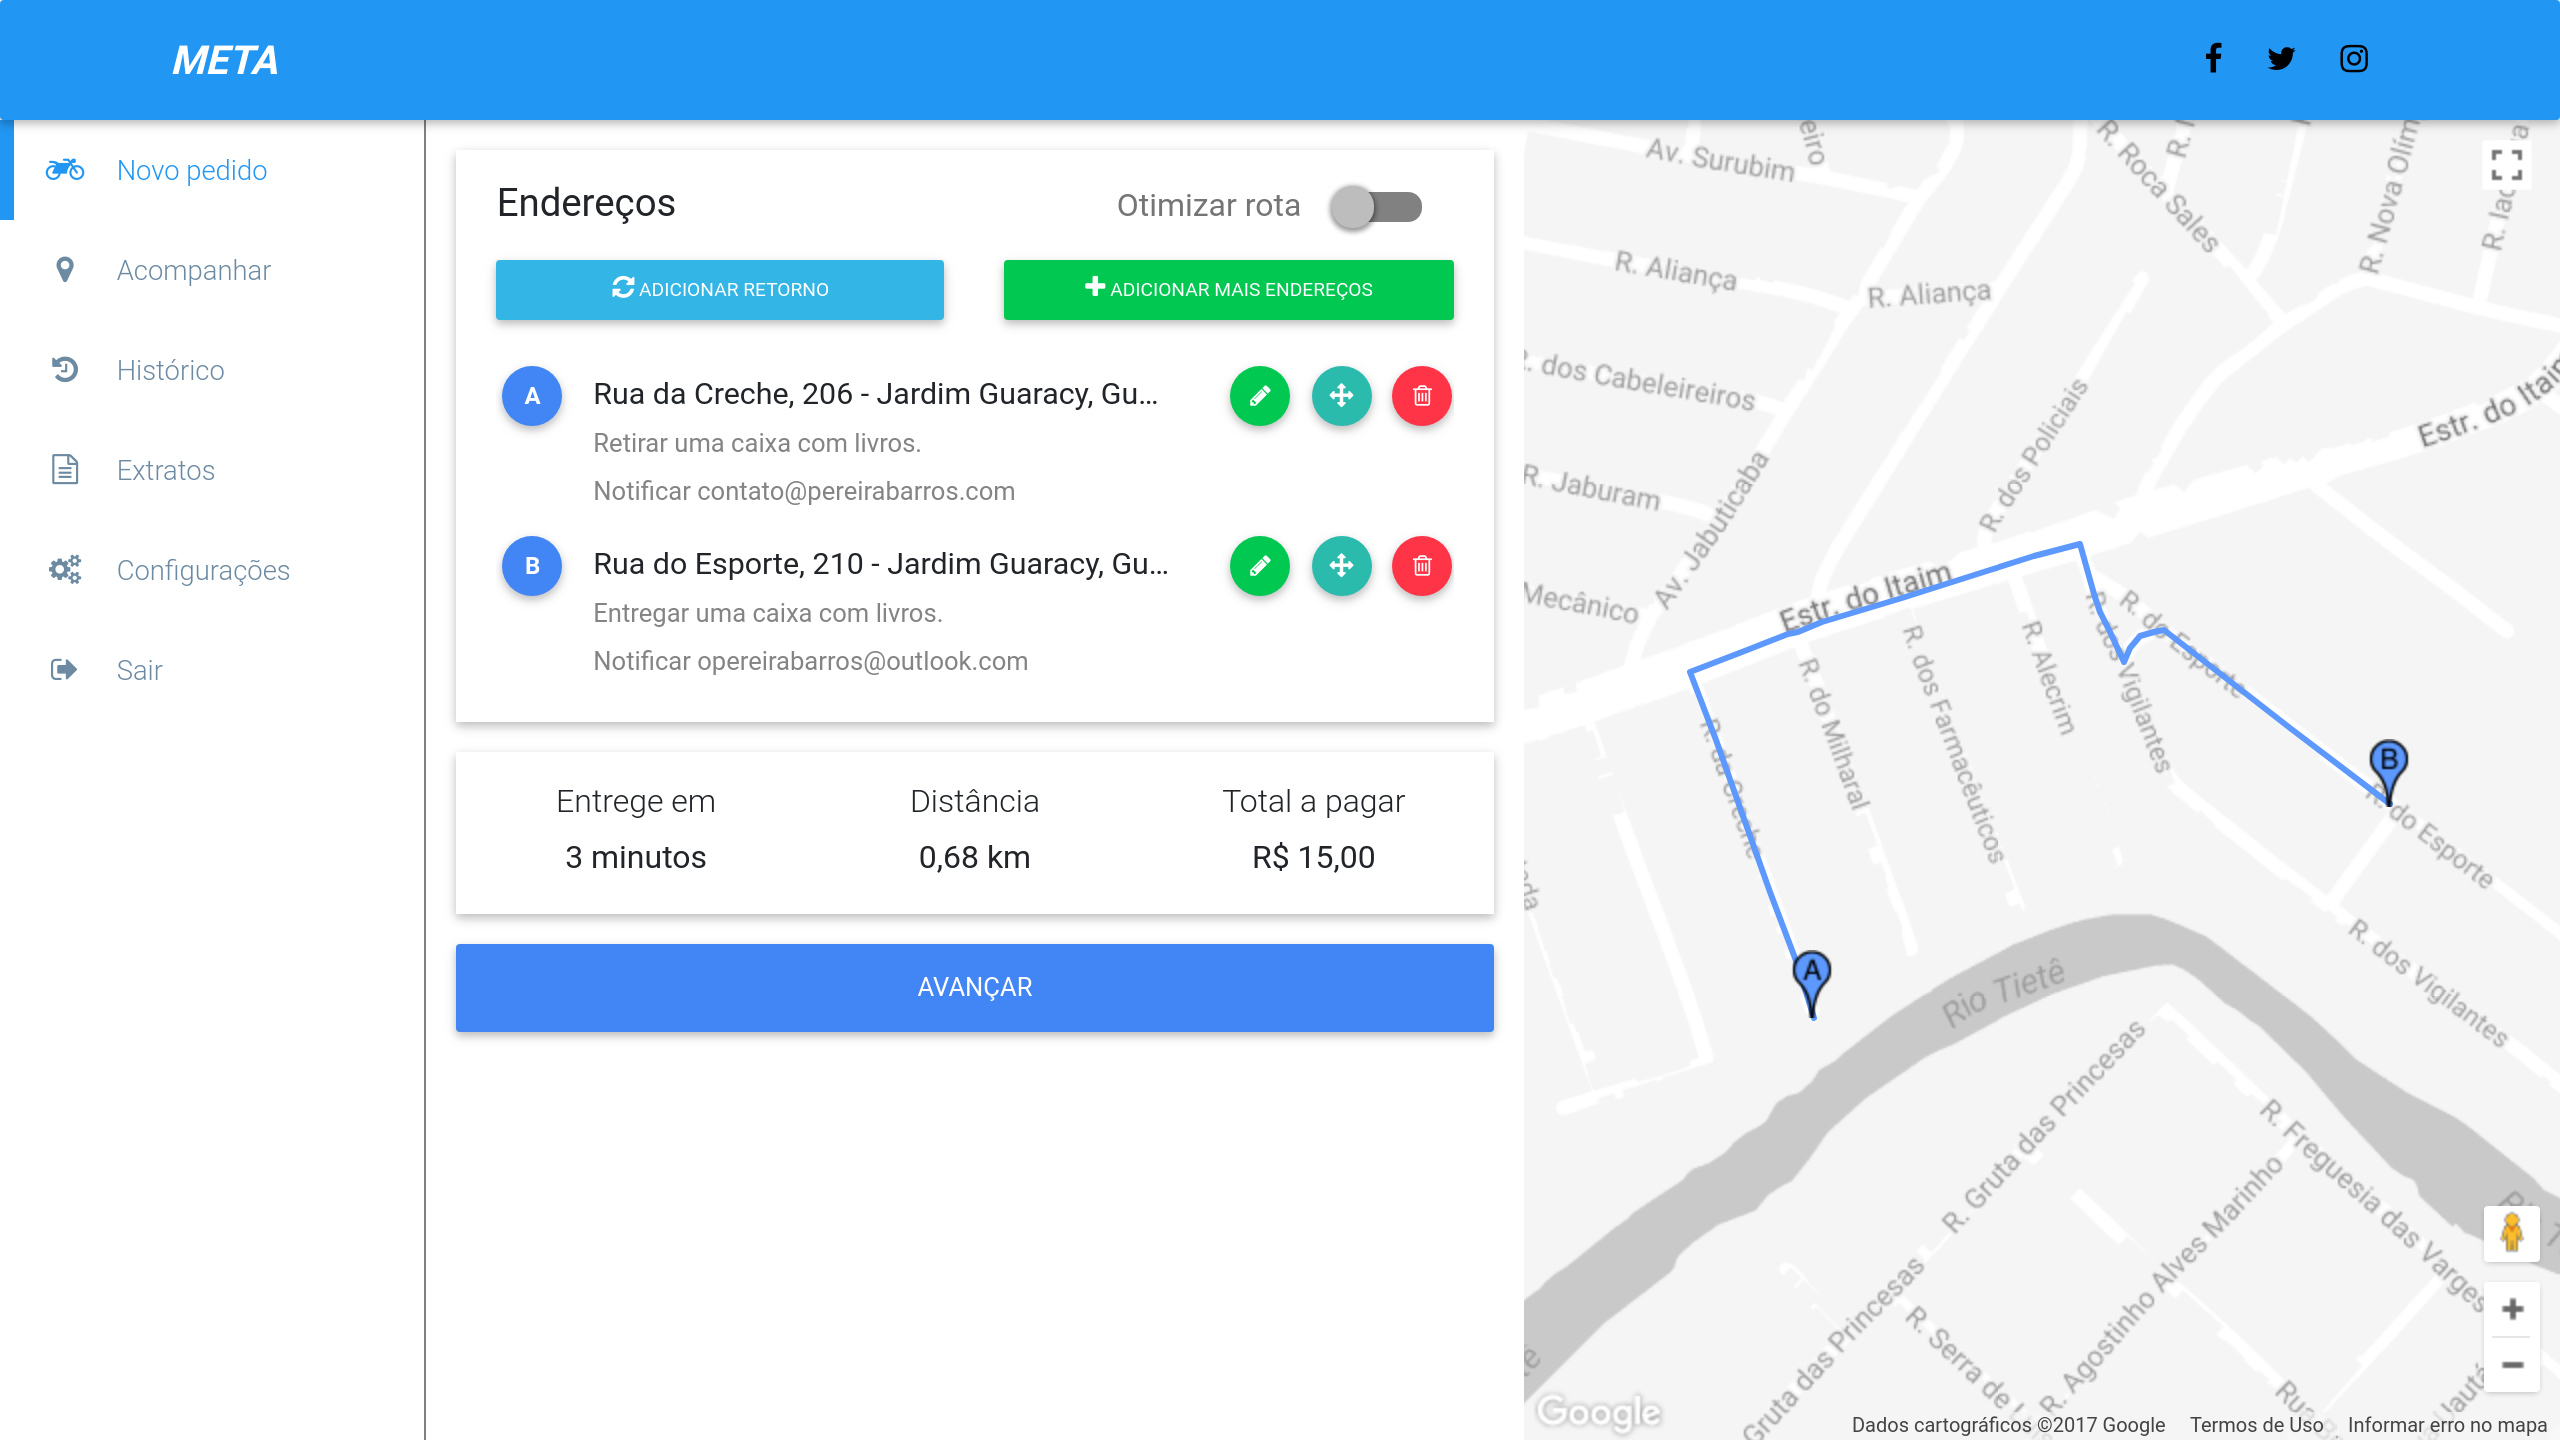
\includegraphics[width=1\textwidth]{./img/depois-entrega}
			\fonte{Captura de tela realizada pelo autor}
			\label{fig:depois-entrega}
		\end{figure}
		
		\begin{figure}[!h]
			\centering
			\caption{Estado da interface de usuário esperada antes da alteração do ponto de retirada}
			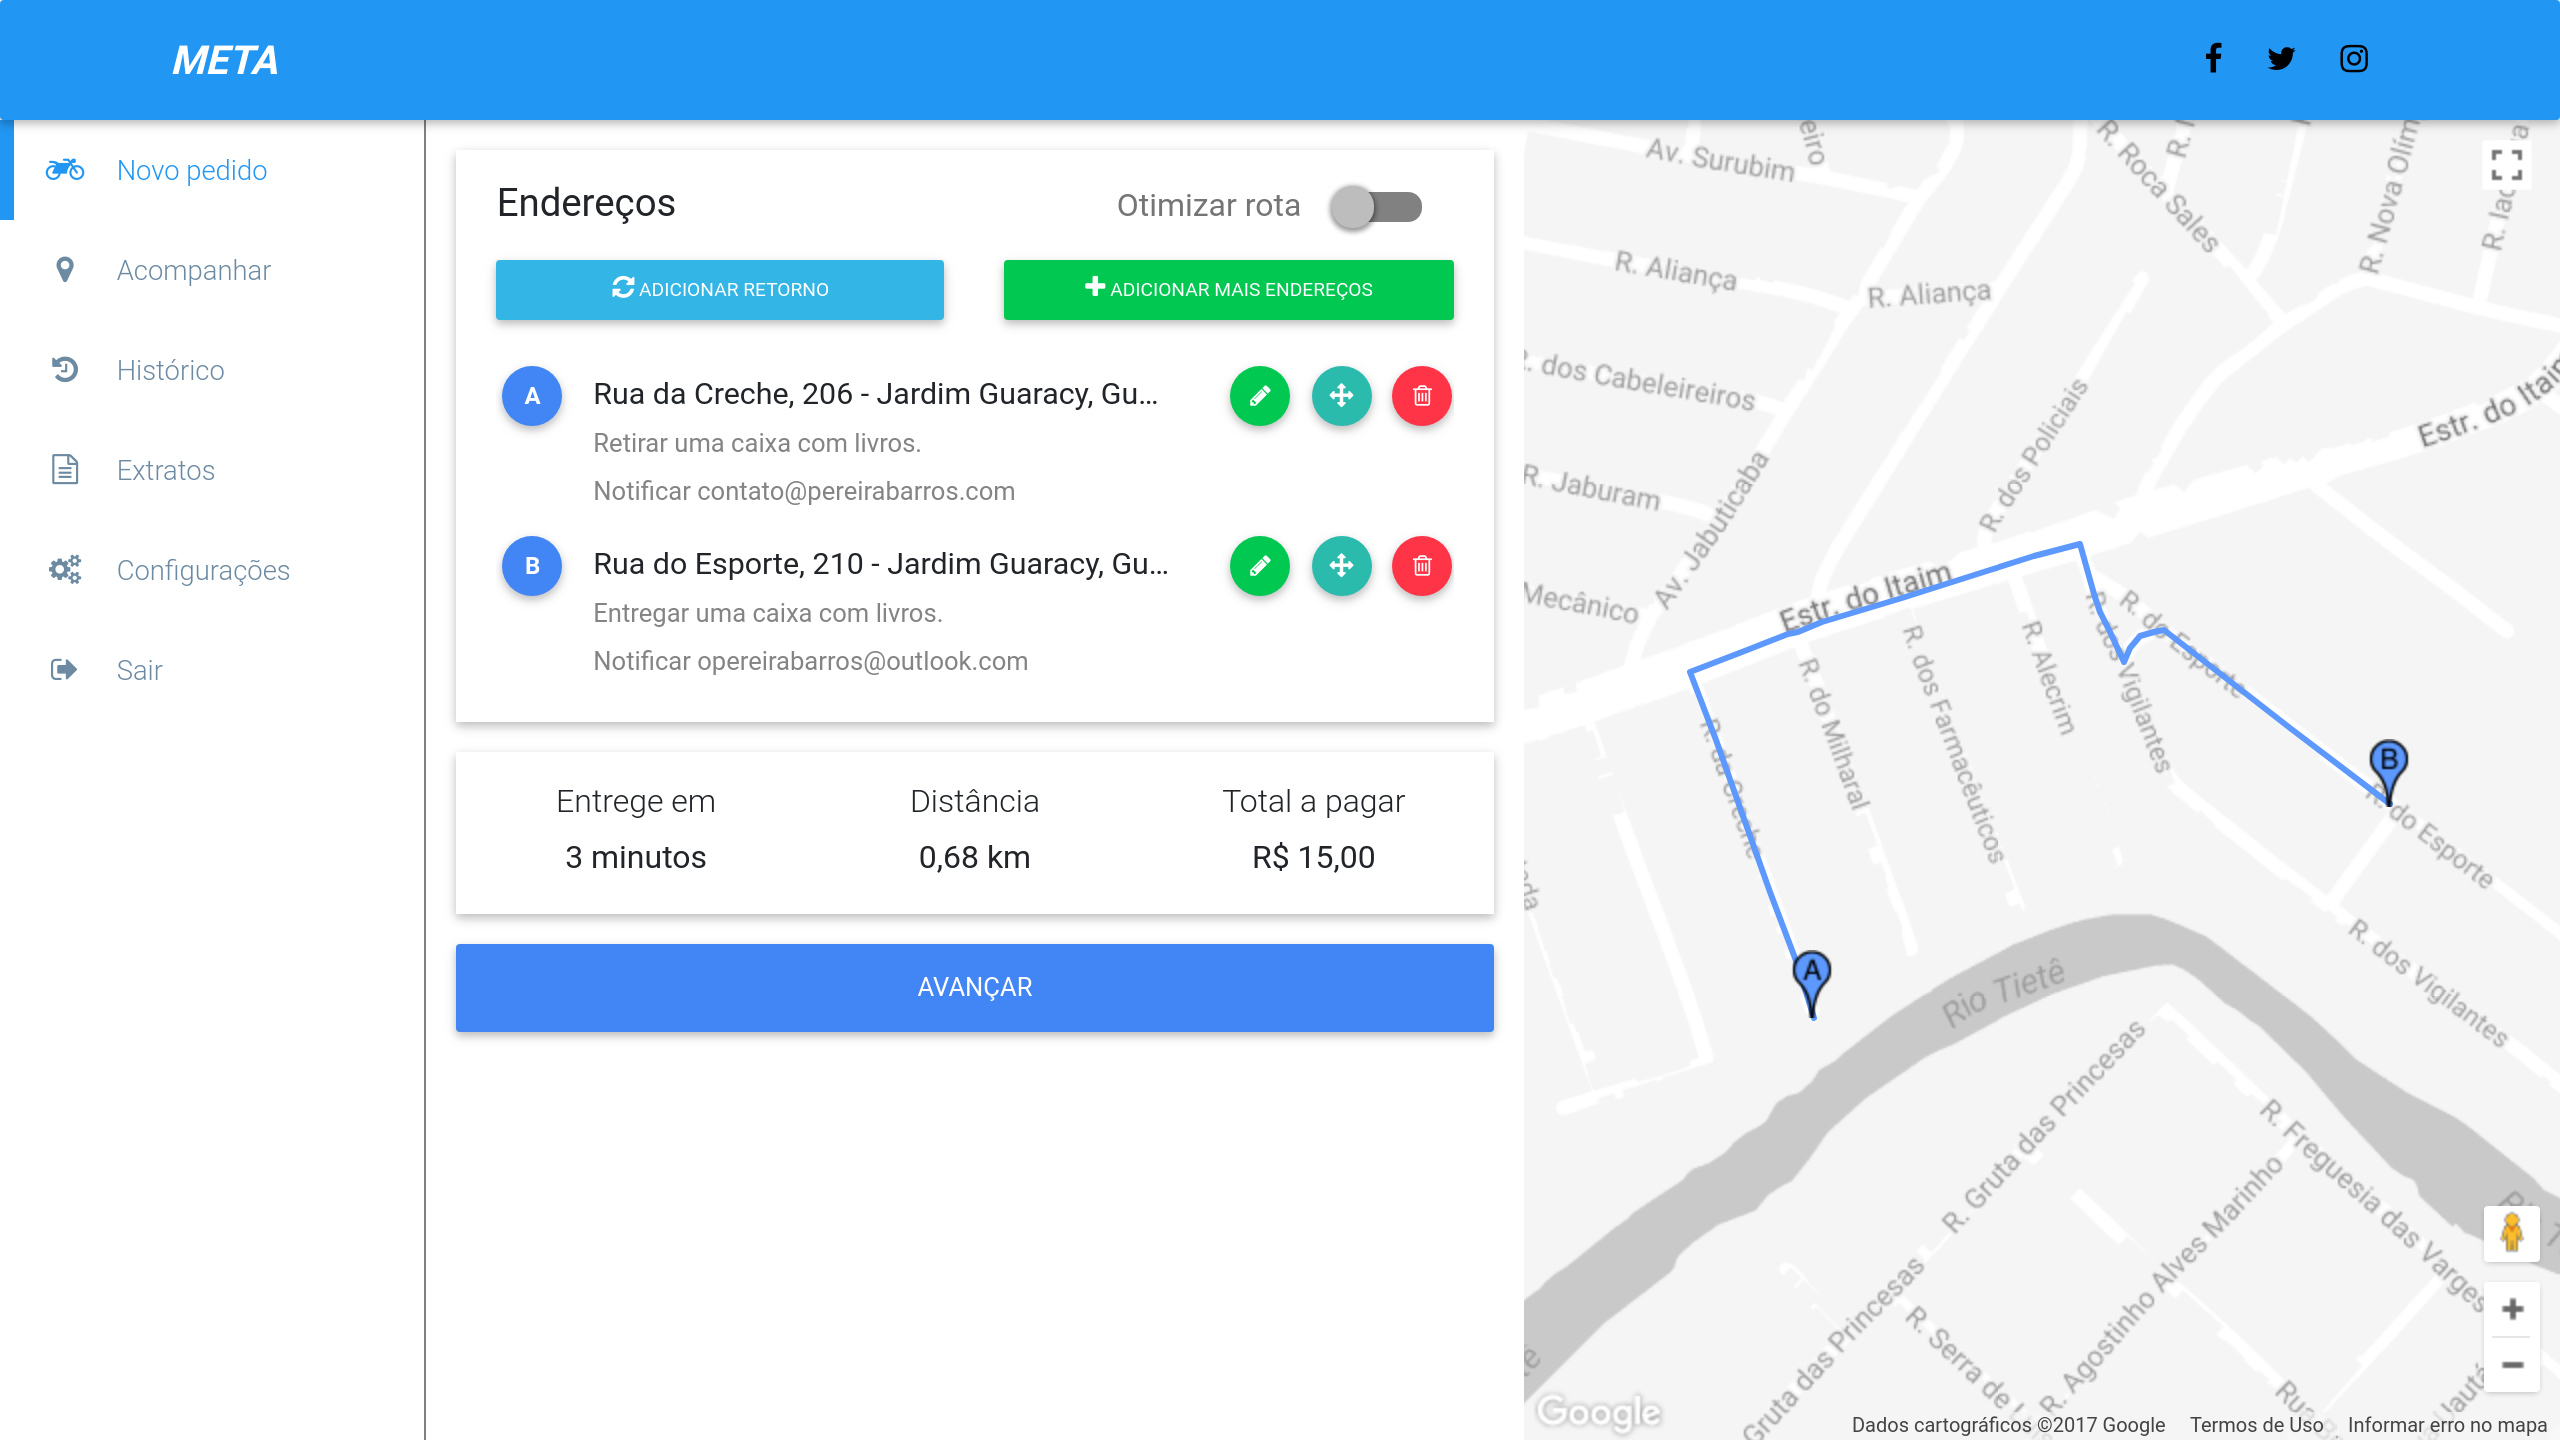
\includegraphics[width=1\textwidth]{./img/depois-entrega}
			\fonte{Captura de tela realizada pelo autor}
			\label{fig:antes-alterar}
		\end{figure}
		
		\begin{figure}[!h]
			\centering
			\caption{Estado da interface de usuário esperada durante da alteração do ponto de retirada}
			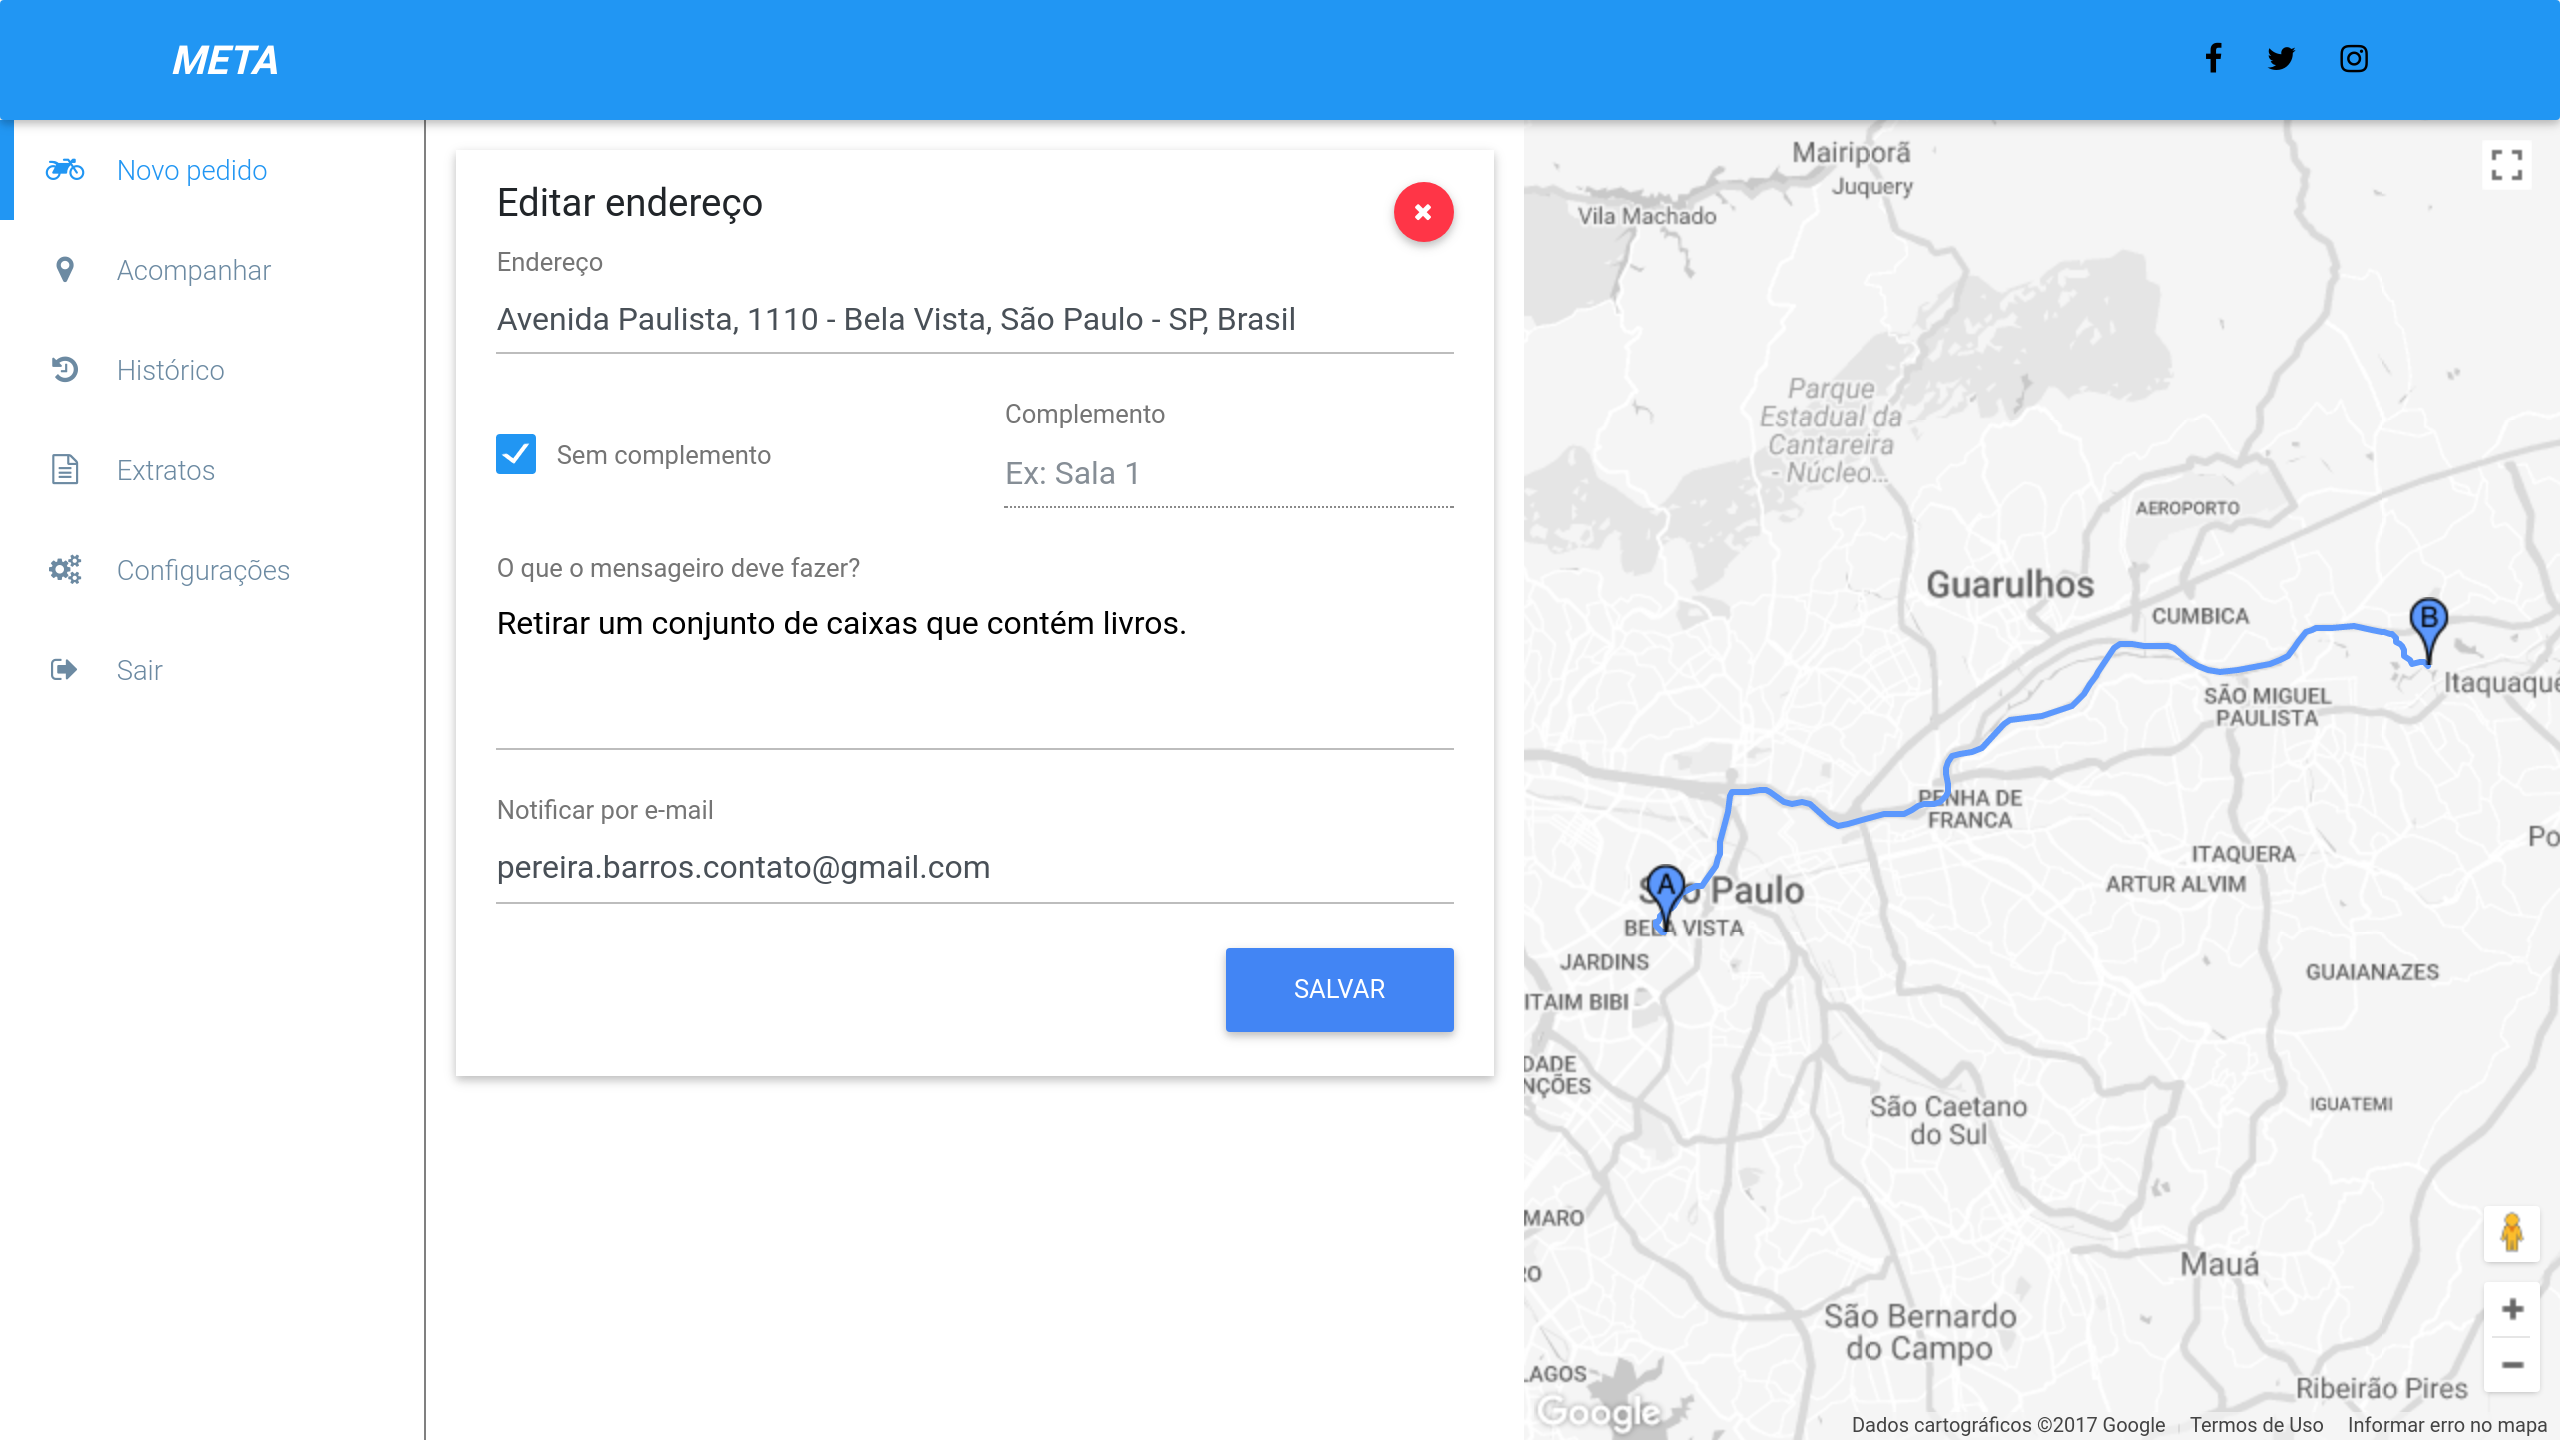
\includegraphics[width=1\textwidth]{./img/durante-alterar}
			\fonte{Captura de tela realizada pelo autor}
			\label{fig:durante-alterar}
		\end{figure}
		
		\begin{figure}[!h]
			\centering
			\caption{Estado da interface de usuário esperada depois da alteração do ponto de retirada}
			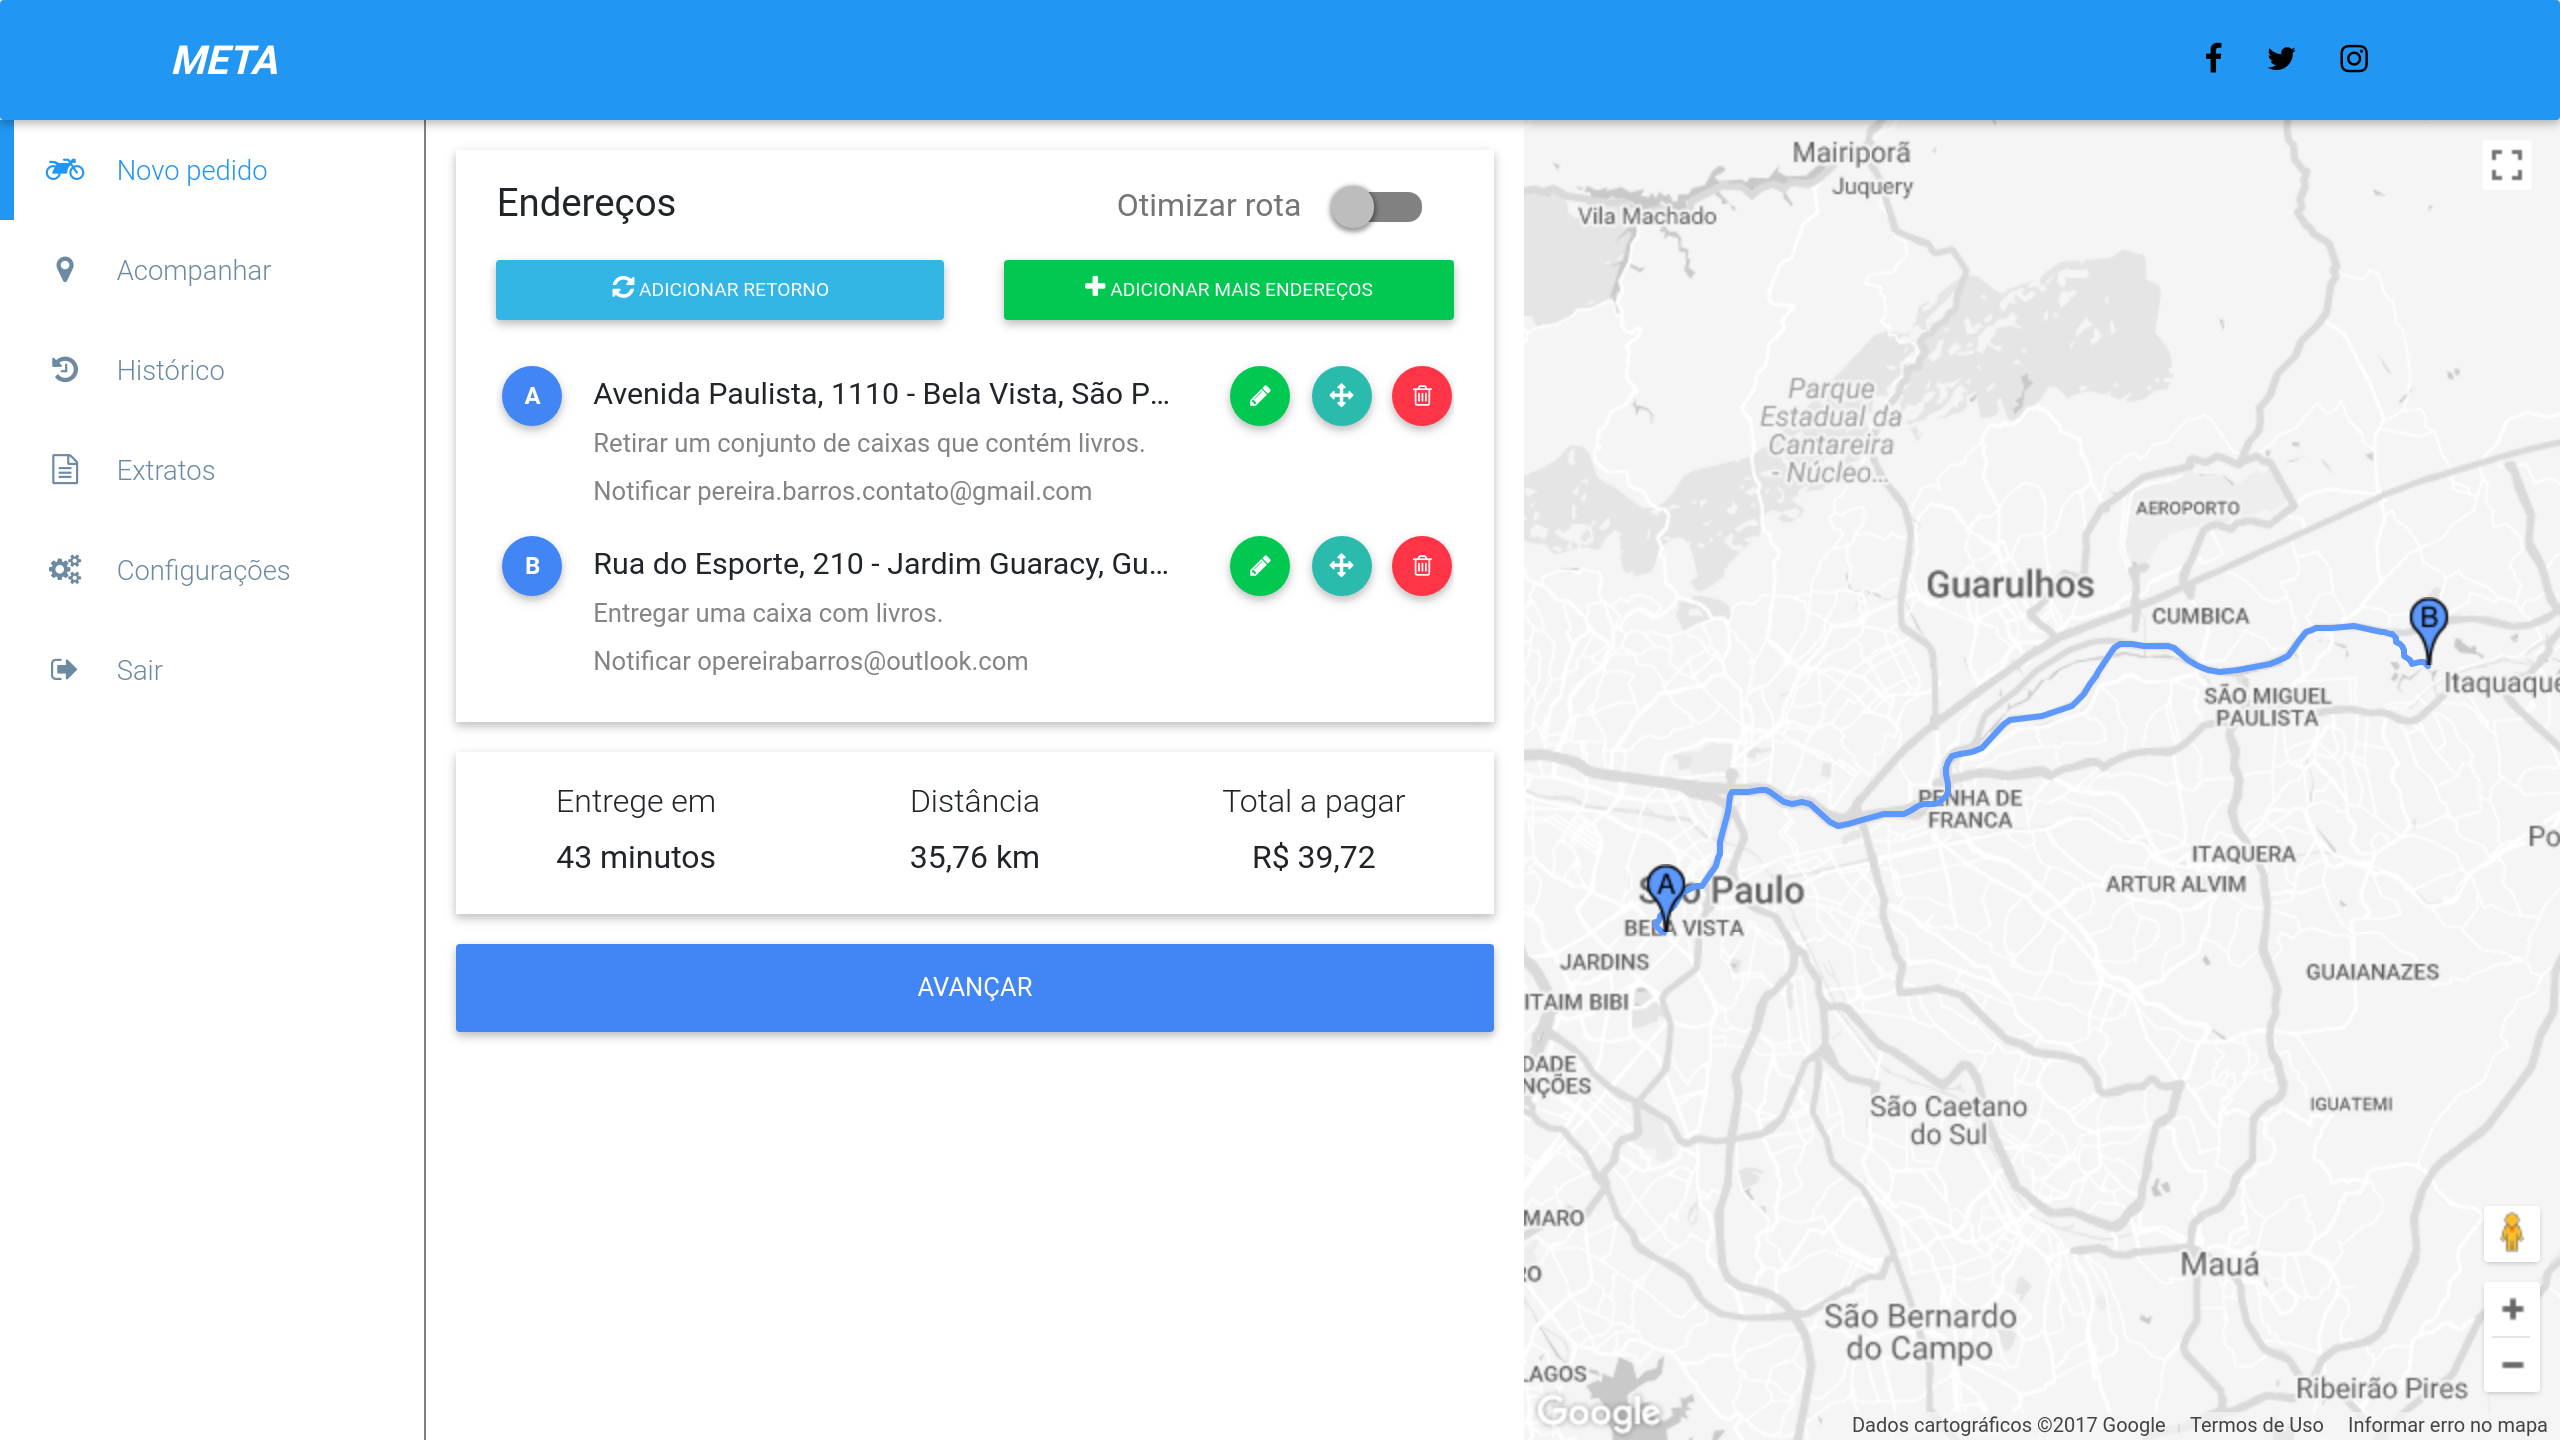
\includegraphics[width=1\textwidth]{./img/depois-alterar}
			\fonte{Captura de tela realizada pelo autor}
			\label{fig:depois-alterar}
		\end{figure}
		
		\begin{figure}[!h]
			\centering
			\caption{Estado da interface de usuário constatada quando o participante esqueceu de informar o número predial do endereço do ponto de retirada}
			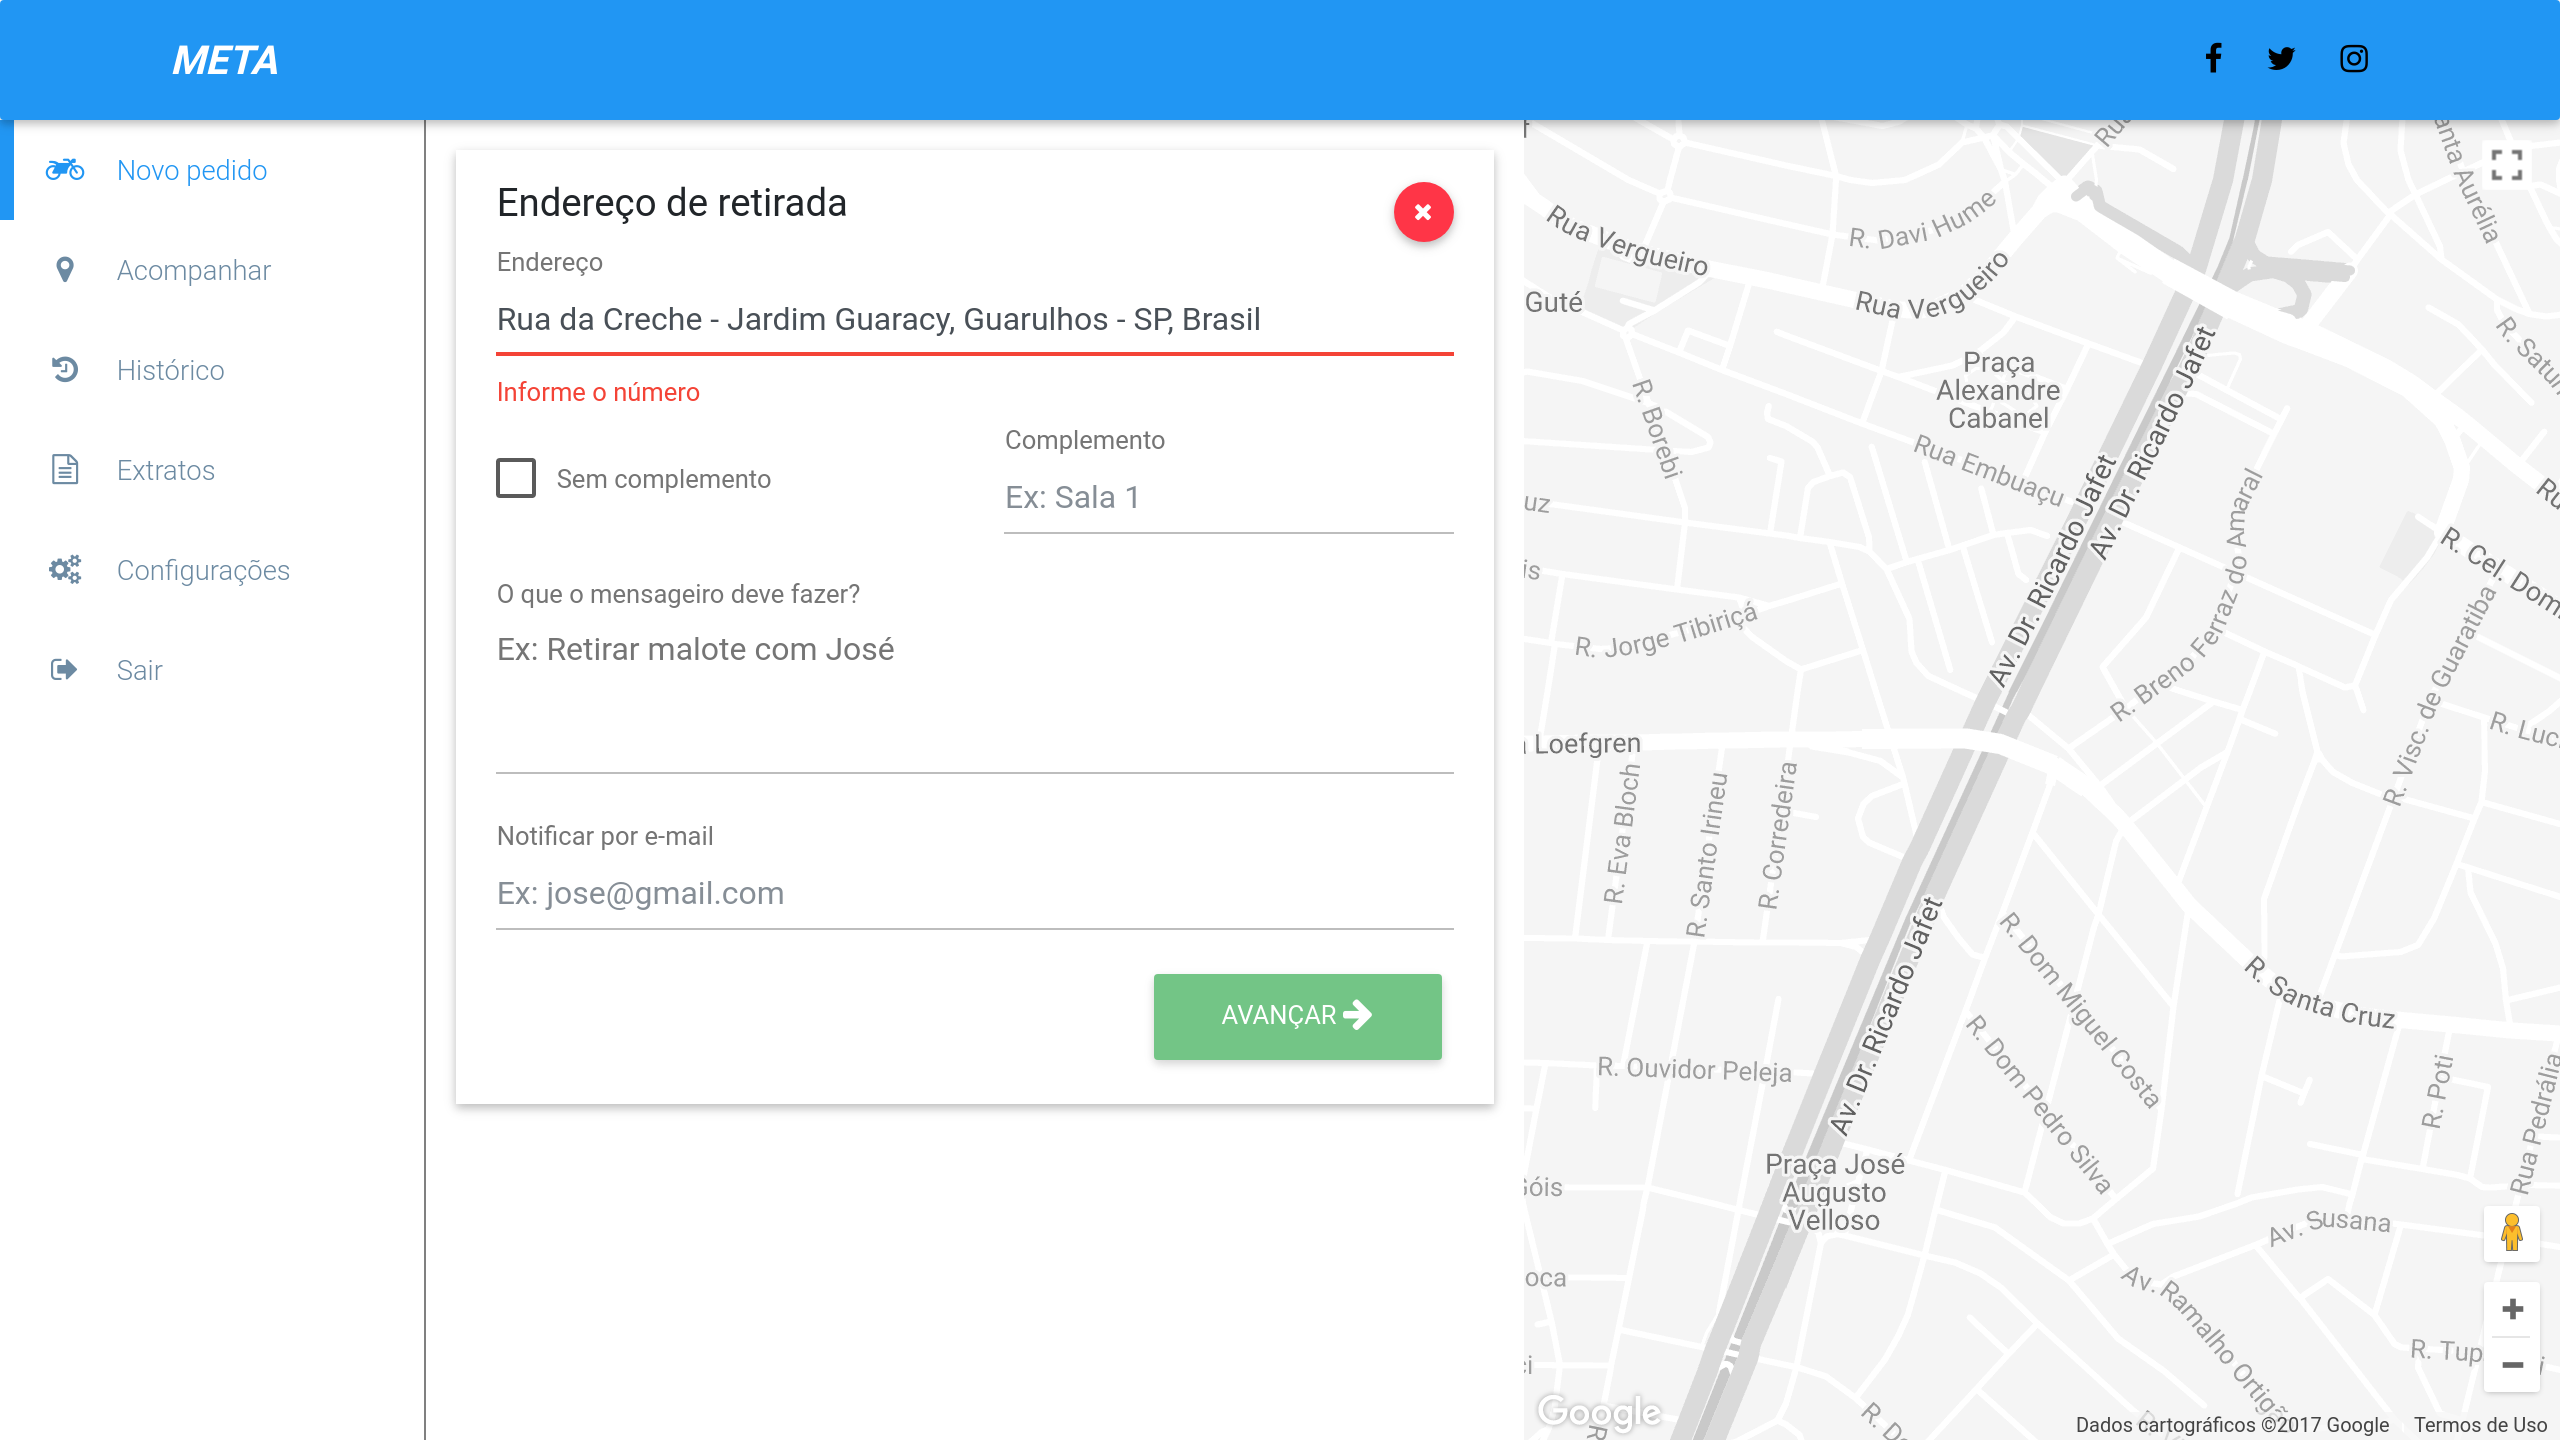
\includegraphics[width=1\textwidth]{./img/falta-numero}
			\fonte{Captura de tela realizada pelo autor}
			\label{fig:falta-numero}
		\end{figure}
		
\end{apendicesenv} 
\bibliography{referencias}
\end{document}